\documentclass[a4paper,12pt]{article}

\usepackage[utf8]{inputenc}
\usepackage{amsmath}
\usepackage{amssymb}
\usepackage{graphicx}
\usepackage{geometry,pdfpages}
\geometry{a4paper, top=1.5cm,bottom=1.5cm,right=2cm,left=1.5cm}
\usepackage{tikz}
\usetikzlibrary{positioning}
\usetikzlibrary{intersections}
\usetikzlibrary{decorations.markings}
\usetikzlibrary{calc}
\usepackage{pgfplots}
\pgfplotsset{width=9cm, compat=1.9}
\usepackage{multicol}
\usepackage{array}
\usepackage[abs]{overpic}
\usepackage{pict2e}
\renewcommand{\baselinestretch}{1.2}
\setlength{\columnsep}{1cm}
\usepackage[inline]{enumitem}
\usepackage{setspace}
\usepackage{subcaption,tcolorbox}
\usepackage{array}
\usepackage{calc}
\usepackage{tcolorbox}
\usepackage[makeroom]{cancel}
\usepackage{hyperref}
\hypersetup{
	colorlinks=true,
	linkcolor=blue,
	filecolor=magenta,      
	urlcolor=cyan,
} 


\newcolumntype{L}[1]{>{\raggedright\let\newline\\\arraybackslash\hspace{0pt}}m{#1}}
\newcolumntype{C}[1]{>{\centering\let\newline\\\arraybackslash\hspace{0pt}}m{#1}}
\newcolumntype{R}[1]{>{\raggedleft\let\newline\\\arraybackslash\hspace{0pt}}m{#1}}
\usepackage{tcolorbox}
\renewcommand{\arraystretch}{1.5}

\setlength\parindent{0pt}
\newcommand{\lineDist}{1}
\newcommand{\lWid}{0}
\definecolor{linecolor}{RGB}{90,90,90}
\definecolor{shadecolor}{RGB}{180,180,180}
\definecolor{backcolor}{RGB}{220,220,220}
\definecolor{whitening}{RGB}{255,255,255}
\newcommand{\numLines}{2}%subtract one
\newcommand{\Qsep}{1}%separation between Question and lines
%-----------------------------
\newcommand\question{
	 \rule[0pt]{17cm}{0.5pt}\vspace{-0.5cm}
	\subsubsection{Exercise}

}
\newcommand\questionend{
	\rule[0pt]{17cm}{0.5pt}\vspace{0.0cm}\\
}
\newcommand\quiz{
\subsubsection{Quiz}\vspace{-0.5cm}
}

\newcommand\boxes[7]{
	\begin{tikzpicture}
	\newcommand{\wid}{1.6cm}
	\newcommand{\hgt}{1cm}
	\newcommand{\brd}{0.4cm}
	\draw[](0,0)rectangle(0+\wid,0+\hgt);
	\draw[](\wid/2,\hgt/2)node[]{\footnotesize #1};
	\draw[](0-\wid/2,0-\hgt)rectangle(0+\wid/2,0);
	\draw[](0,-\hgt/2)node[]{\footnotesize #2};
	\draw[](0+\wid/2,0-\hgt)rectangle(0+3*\wid/2,0);
	\draw[](\wid,-\hgt/2)node[]{\footnotesize #3};
	\draw[](0-\wid,0-2*\hgt)rectangle(0,-\hgt);
	\draw[](-\wid/2,-3*\hgt/2)node[]{\footnotesize #4};
	\draw[](0,0-2*\hgt)rectangle(\wid,-\hgt);
	\draw[](\wid/2,-3*\hgt/2)node[]{\footnotesize #5};
	\draw[](0+\wid,0-2*\hgt)rectangle(2*\wid,-\hgt);
	\draw[](3*\wid/2,-3*\hgt/2)node[]{\footnotesize #6};
	\draw[white](-\wid-\brd,-2*\hgt-\brd)rectangle(2*\wid+\brd,\hgt+\brd);
	\draw[](-\wid-\brd,\hgt+\brd)node[anchor= north west]{\textbf{#7)}};
	\end{tikzpicture}
}

\newcommand\boxesSol[7]{
	\begin{tikzpicture}
	\newcommand{\wid}{1.6cm}
	\newcommand{\hgt}{1cm}
	\newcommand{\brd}{0.4cm}
	\draw[](0,0)rectangle(0+\wid,0+\hgt);
	\draw[](\wid/2,\hgt/2)node[]{\footnotesize #1};
	\draw[](0-\wid/2,0-\hgt)rectangle(0+\wid/2,0);
	\draw[](0,-\hgt/2)node[]{\footnotesize #2};
	\draw[](0+\wid/2,0-\hgt)rectangle(0+3*\wid/2,0);
	\draw[](\wid,-\hgt/2)node[]{\footnotesize #3};
	\draw[](0-\wid,0-2*\hgt)rectangle(0,-\hgt);
	\draw[](-\wid/2,-3*\hgt/2)node[]{\footnotesize #4};
	\draw[](0,0-2*\hgt)rectangle(\wid,-\hgt);
	\draw[](\wid/2,-3*\hgt/2)node[]{\footnotesize #5};
	\draw[](0+\wid,0-2*\hgt)rectangle(2*\wid,-\hgt);
	\draw[](3*\wid/2,-3*\hgt/2)node[]{\footnotesize #6};
	\draw[white](-\wid-\brd,-2*\hgt-\brd)rectangle(2*\wid+\brd,\hgt+\brd);
	\draw[](-\wid-\brd,\hgt+\brd)node[anchor= north west]{\textbf{#7)}};
	\end{tikzpicture}
}

\newcommand\addagon[7]{
	\begin{tikzpicture}[scale=1]
	\draw[white](-3,0)rectangle(3,5.5);
	\draw[](-3,4)node[right]{#7)};
		\begin{scope}[scale=0.75]
	\coordinate (A) at (-2.5,1);
	\coordinate (B) at (2.5,1);
	\coordinate (C) at (0,{2.5*sqrt(3)+1});
	\draw[thick](A)--(B)--(C)--(A);
	\foreach \n in {A,B,C}{
		\filldraw[fill=white, draw=black](\n )circle[radius=1cm];
	}
	\draw[](A)node[above, yshift=-9pt]{#1};
	\draw[](B)node[above, yshift=-9pt]{#2};
	\draw[](C)node[above, yshift=-9pt]{#3};
	
	\coordinate (A') at ( $ (A)!0.5!(B) $ );
	\draw[fill=backcolor, draw=black]([shift=(35:-1.2)]A')rectangle([shift=(35:1.2)]A');
	\draw[](A')node[above, yshift=-9pt]{#4};
	
	\coordinate (B') at ( $ (B)!0.5!(C) $ );
	\draw[fill=backcolor, draw=black]([shift=(35:-1.2)]B')rectangle([shift=(35:1.2)]B');
	\draw[](B')node[above, yshift=-9pt]{#5};
	
	\coordinate (C') at ( $ (C)!0.5!(A) $ );
	\draw[fill=backcolor, draw=black]([shift=(35:-1.2)]C')rectangle([shift=(35:1.2)]C');
	\draw[](C')node[above, yshift=-9pt]{#6};
		\end{scope}
	\end{tikzpicture}
}

\newcommand\addagonSol[7]{
	\begin{tikzpicture}[scale=1]
	\draw[white](-3,0)rectangle(3,5.5);
	\draw[](-3,4)node[right]{#7)};
	\begin{scope}[scale=0.75]
	\coordinate (A) at (-2.5,1);
	\coordinate (B) at (2.5,1);
	\coordinate (C) at (0,{2.5*sqrt(3)+1});
	\draw[thick](A)--(B)--(C)--(A);
	\foreach \n in {A,B,C}{
		\filldraw[fill=white, draw=black](\n )circle[radius=1cm];
	}
	\draw[](A)node[above, yshift=-9pt]{#1};
	\draw[](B)node[above, yshift=-9pt]{#2};
	\draw[](C)node[above, yshift=-9pt]{#3};
	
	\coordinate (A') at ( $ (A)!0.5!(B) $ );
	\draw[fill=backcolor, draw=black]([shift=(35:-1.2)]A')rectangle([shift=(35:1.2)]A');
	\draw[](A')node[above, yshift=-9pt]{#4};
	
	\coordinate (B') at ( $ (B)!0.5!(C) $ );
	\draw[fill=backcolor, draw=black]([shift=(35:-1.2)]B')rectangle([shift=(35:1.2)]B');
	\draw[](B')node[above, yshift=-9pt]{#5};
	
	\coordinate (C') at ( $ (C)!0.5!(A) $ );
	\draw[fill=backcolor, draw=black]([shift=(35:-1.2)]C')rectangle([shift=(35:1.2)]C');
	\draw[](C')node[above, yshift=-9pt]{#6};
	\end{scope}
	\end{tikzpicture}
}


\newcommand\sumproduct[5]{
\begin{tikzpicture}[scale=0.6]
\draw[white](-4.75,-2.75)rectangle(4.75,5);
\draw[](-4.5,4.5)node[right, yshift=-0.2cm]{\footnotesize \textbf{#5)}};
\draw[](-4,0)rectangle(0,2);
\draw[](0,0)rectangle(4,2);
\draw[](-2,2)rectangle(2,4);
\draw[](-2,-2)rectangle(2,0);
\draw[](0,-1)node[]{#1};
\draw[](0,3)node[]{#2};
\draw[](-2,1)node[]{#3};
\draw[](2,1)node[]{#4};
\draw[](-4,3)node[right]{\tiny Product:};
\draw[](-4,-1)node[right]{\tiny Sum:};
\end{tikzpicture}
}
\newcommand\sumproductSol[5]{
	\begin{tikzpicture}[scale=0.6]
	\draw[white](-4.75,-2.75)rectangle(4.75,5);
	\draw[](-4.5,4.5)node[right, yshift=-0.2cm]{\footnotesize \textbf{#5)}};
	\draw[](-4,0)rectangle(0,2);
	\draw[](0,0)rectangle(4,2);
	\draw[](-2,2)rectangle(2,4);
	\draw[](-2,-2)rectangle(2,0);
	\draw[](0,-1)node[]{#1};
	\draw[](0,3)node[]{#2};
	\draw[](-2,1)node[]{#3};
	\draw[](2,1)node[]{#4};
	\draw[](-4,3)node[right]{\tiny Product:};
	\draw[](-4,-1)node[right]{\tiny Sum:};
	\end{tikzpicture}
}

%-----------------------------
\begin{document}
	\thispagestyle{empty}
	\LARGE
\textbf{Name / Ingoa}  \rule[0pt]{12cm}{0.5pt}\\
\begin{center}
	\textbf{Year 10 Pāngarau (Mathematics)}
\end{center}
\begin{figure}[!h]
	\centering
	
\includegraphics[width=10cm]{other_graphics/marsden_black_white.jpg}
\end{figure}
\begin{center}
	\textbf{Algebra: Expressions and Equations}
\end{center}

\begin{figure}[!h]
	\centering
	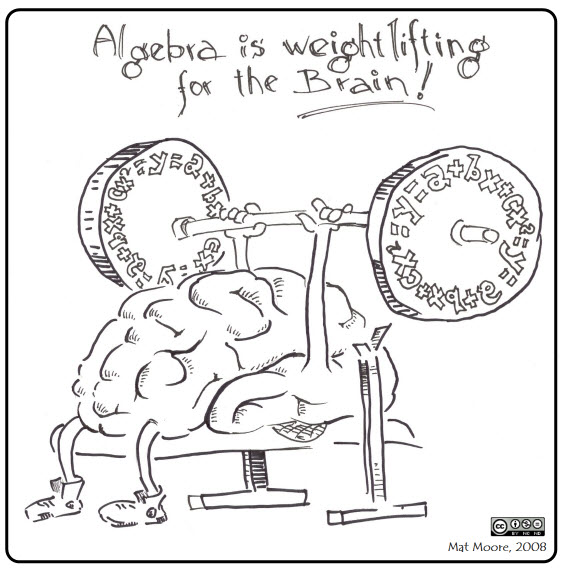
\includegraphics[width=10cm]{other_graphics/algebra_weightlifting.jpeg}
\end{figure}

\normalsize
	\newpage
	\setcounter{tocdepth}{2}
	\tableofcontents
	\newpage


%\LARGE
	% ------------------
\section{Substitution}
 %\rule[-1pt]{5cm}{0.5pt}
\question
If $c=5$ evaluate the following expressions
\begin{multicols}{2}
	\begin{enumerate}[label=\normalsize \alph*)~~~ , topsep=8pt,itemsep=5pt,partopsep=4pt, parsep=4pt]
		\item $c+c+c$
		\item $4c$
		\item $c^2$
		\item $c^3$
		\item $3c-8$
		\item $-4c^2$
	\end{enumerate}
\end{multicols}\vspace{0.2cm}
\question
If $b=-3$ evaluate the following expressions
\begin{multicols}{2}
	\begin{enumerate}[label=\normalsize \alph*)~~~ , topsep=8pt,itemsep=5pt,partopsep=4pt, parsep=4pt]
		\item $2b$
		\item $b +9$
		\item $-4b$
		\item $b \times b$
		\item $b^2$
		\item $b^3$
		\item $b^4$
		\item $3b+8$
	\end{enumerate}
\end{multicols}\vspace{0.2cm}
\question
If $x=7$ and $y=-2$ evaluate the following expressions
\begin{multicols}{2}
	\begin{enumerate}[label=\normalsize \alph*)~~~ , topsep=8pt,itemsep=5pt,partopsep=4pt, parsep=4pt]
		\item $x+y+x+y+x+y+x$
		\item $4x +3y$
		\item $x+4+x$
		\item $x^2 + 2y$
		\item $x^2 + y+y+y+x^2$
		\item $2x^2 +3y$
	\end{enumerate}
\end{multicols}\vspace{0.2cm}
\questionend
\newpage
\section{Adding and Subtracting with numbers}
\subsection{Addition}
\textbf{Addition} is commutative.\\
The means that we can reorder an addition any way we like.\\
For example: $2+6+1+2+6 =  1 +2+2+6+6$\\\\
For the questions below: 
\begin{itemize}
	\item Reorder the addition into order from smallest to largest numbers
	\item Evaluate each group of the same number
	\item Then complete the addition
\end{itemize}
Example: Re order and calculate: $9+2+3+9+9+2+9+3$
\begin{align*}
	&=  2 + 2 + 3+3 +9+9+9\\
	&=  2 \times 2 + 2 \times 3 + 3 \times 9 \\
	&= 4 + 6 +27\\
	& = 37
\end{align*}
\question
Re order and calculate:
\begin{multicols}{2}
	\begin{enumerate}[label=\normalsize \alph*)~~~ , topsep=8pt,itemsep=5pt,partopsep=4pt, parsep=4pt]
		\item $4+7+7+2+7+4$
		\item $12 + 6 + 4 + 12 +4 +6 +4$
		\item $11 +2+ 11 +2 + 11 +2 +2$
		\item $13 + 10 +  3 + 10 + 13 + 3+ 3 +3$
	\end{enumerate}
\end{multicols}\vspace{0.2cm}
\questionend
Example for the next set:\\
Re order and calculate: $4+2 \times 7+2+7+3 \times 4$
\begin{align*}
	&=  2 + 4  +3 \times 4 + 7 + 2 \times 7 \\
	&=  2 + 4 \times 4 + 3 \times 7 \\
	&= 4 + 16 +21\\
	& = 41
\end{align*}
\newpage
\question
Re order and calculate:
\begin{multicols}{2}
	\begin{enumerate}[label=\normalsize \alph*)~~~ , topsep=8pt,itemsep=5pt,partopsep=4pt, parsep=4pt]
		\item $4+9+3 \times 9 +7+7+2 \times4$
		\item $2 \times 12 + 5 + 5 + 12 + 3 \times 5  +4$
		\item $3\times 11 +2+ 2\times11 +2 + 11 +3 \times 2 +2$
		\item $2 \times 13 + 10 +  13 + 5 \times 10 + 13 + 4 +4$
	\end{enumerate}
\end{multicols}\vspace{0.2cm}
\questionend
\subsection{Addition and Subtraction}
We can do the reordering with subtractions as well , but we have to \textbf{think}.\\
The sign to the left of the number , moves with the number.\\\\
For example : $5 - 8 = -8 +5 $  (there is an invisible $+$ left of the $5$)\\\\
For a longer sum, for example: $4 -5+4+5 +4 -5$
\begin{itemize}
	\item We can `split' it as : $|~+4|~ -5|~+4|~+5|~ +4|~ -5|$
	\item Then reorder: $+4 + 4 + 4 +5 -5 -5 = 3\times 4 -5 = 7$
\end{itemize}
\question
Re order and calculate:
\begin{multicols}{2}
	\begin{enumerate}[label=\normalsize \alph*)~~~ , topsep=8pt,itemsep=5pt,partopsep=4pt, parsep=4pt]
		\item $4-9 +4-9+4 + 4$
		\item $8 -1 -1 +8 -1+8 $
		\item $-7 -2 -2 -7 -7$
		\item $-2 \times 6 - 3 \times 2  -6  -2$
		\item $3\times 11 +2-2\times11 +11 -3 \times 2 $
		\item $-2 \times 13 + 5 \times 10 + 13 -2\times 10$
	\end{enumerate}
\end{multicols}\vspace{0.2cm}
\questionend
\newpage

\section{Adding and Subtracting Like Terms}
%\LARGE
When using algebra, the different letters represent (most likely) different numbers so we can re order and simplify algebra expressions , using the techniques used above.\\\\
Examples:
\begin{multicols}{2}
	~\vspace{-1.1cm}
	\begin{align*}
		& x+ y +x + y+ y\\
		&=  x + x + y + y+y\\
		&= 2x + 3y\\
	\end{align*}
	\begin{align*}
		& 2y +x + 3y + x+ x\\
		&=  x + x+x+ 2y+3y\\
		&= 3x + 5y\\
	\end{align*}
\end{multicols}
\question
Simplify the following expressions.
\begin{multicols}{2}
	\begin{enumerate}[label=\normalsize \alph*)~~~ , topsep=8pt,itemsep=5pt,partopsep=4pt, parsep=4pt]
		\item $x+4+x$
		\item $y+y+y+y$
		\item $x+y+x+x$
		\item $2x+3y+4x +5y +3$
		\item $5x+y + 3x+6y$
		\item $7y +y +x+5x -8$
	\end{enumerate}
\end{multicols}\vspace{0.2cm}
\questionend
Examples:
\begin{multicols}{2}
	~\vspace{-1cm}
	\begin{align*}
		& -2x - 3x\\
		&= -5x\\\\
	\end{align*}
	\begin{align*}
		& 2y+3x +6y -4x\\
		&=  3x - 4x + 2y +6y\\
		&= -x + 8y\\
	\end{align*}
\end{multicols}
\question
Simplify the following expressions.
\begin{multicols}{2}
	\begin{enumerate}[label=\normalsize \alph*)~~~ , topsep=8pt,itemsep=5pt,partopsep=4pt, parsep=4pt]
		\item $-7x - 4x$
		\item $2y -7x +3y - 4x$
		\item $2x-3+3y-4x +5y+1$
		\item $-5x+y-3x+6y$
		\item $-7y +y +x+5x -8$
		\item $-8y +3z -4x- 8 +5x -7y$
	\end{enumerate}
\end{multicols}\vspace{0.2cm}
\questionend
\newpage
If we have a power with an algebra letter (e.g. $x^2$) then we cannot 'add' this with the $x$ terms (because it will evaluate to a different number than $x$).\\\\
This means that: $x+ x + x^2 = 2x + x^2$\\\\
Or that $x^2 + y +2y^2 + 2y + 3y^2 = x^2 + 3y + 5y^2 $\\
\question
Simplify the following expressions.
\begin{multicols}{2}
	\begin{enumerate}[label=\normalsize \alph*)~~~, topsep=8pt,itemsep=12pt,partopsep=4pt, parsep=4pt]
		\item $x^2+x+x^2+x^2+x+x$
		\item $y+y^2+y^2-2y-3y$
		\item $3y^2+2y-6y^2$
		\item $2x^2+3y^2-4x +5y^2$
		\item $-5x^2+y-8x^2+6y$
		\item $-7y^2 +y^2+y+5y -3$
	\end{enumerate}
\end{multicols}\vspace{0.2cm}
\questionend
\subsection{Mixed Questions}
\question
Simplify the following expressions.
\begin{multicols}{2}
	\begin{enumerate}[label=\normalsize \alph*)~~~, topsep=8pt,itemsep=12pt,partopsep=4pt, parsep=4pt]
		\item $2x+4+5x$
		\item $y+9-6y+2$
		\item $x^2+2x+x^2+1$
		\item $2x^2-5x+x^2-x$
		\item $-5x+y-3x+x^2$
		\item $x^2-y^2-x^2+2y^2$
	\end{enumerate}
\end{multicols}
\questionend
% ------------------------------
\newpage
\quiz
\begin{figure}[!h]
	\centering
	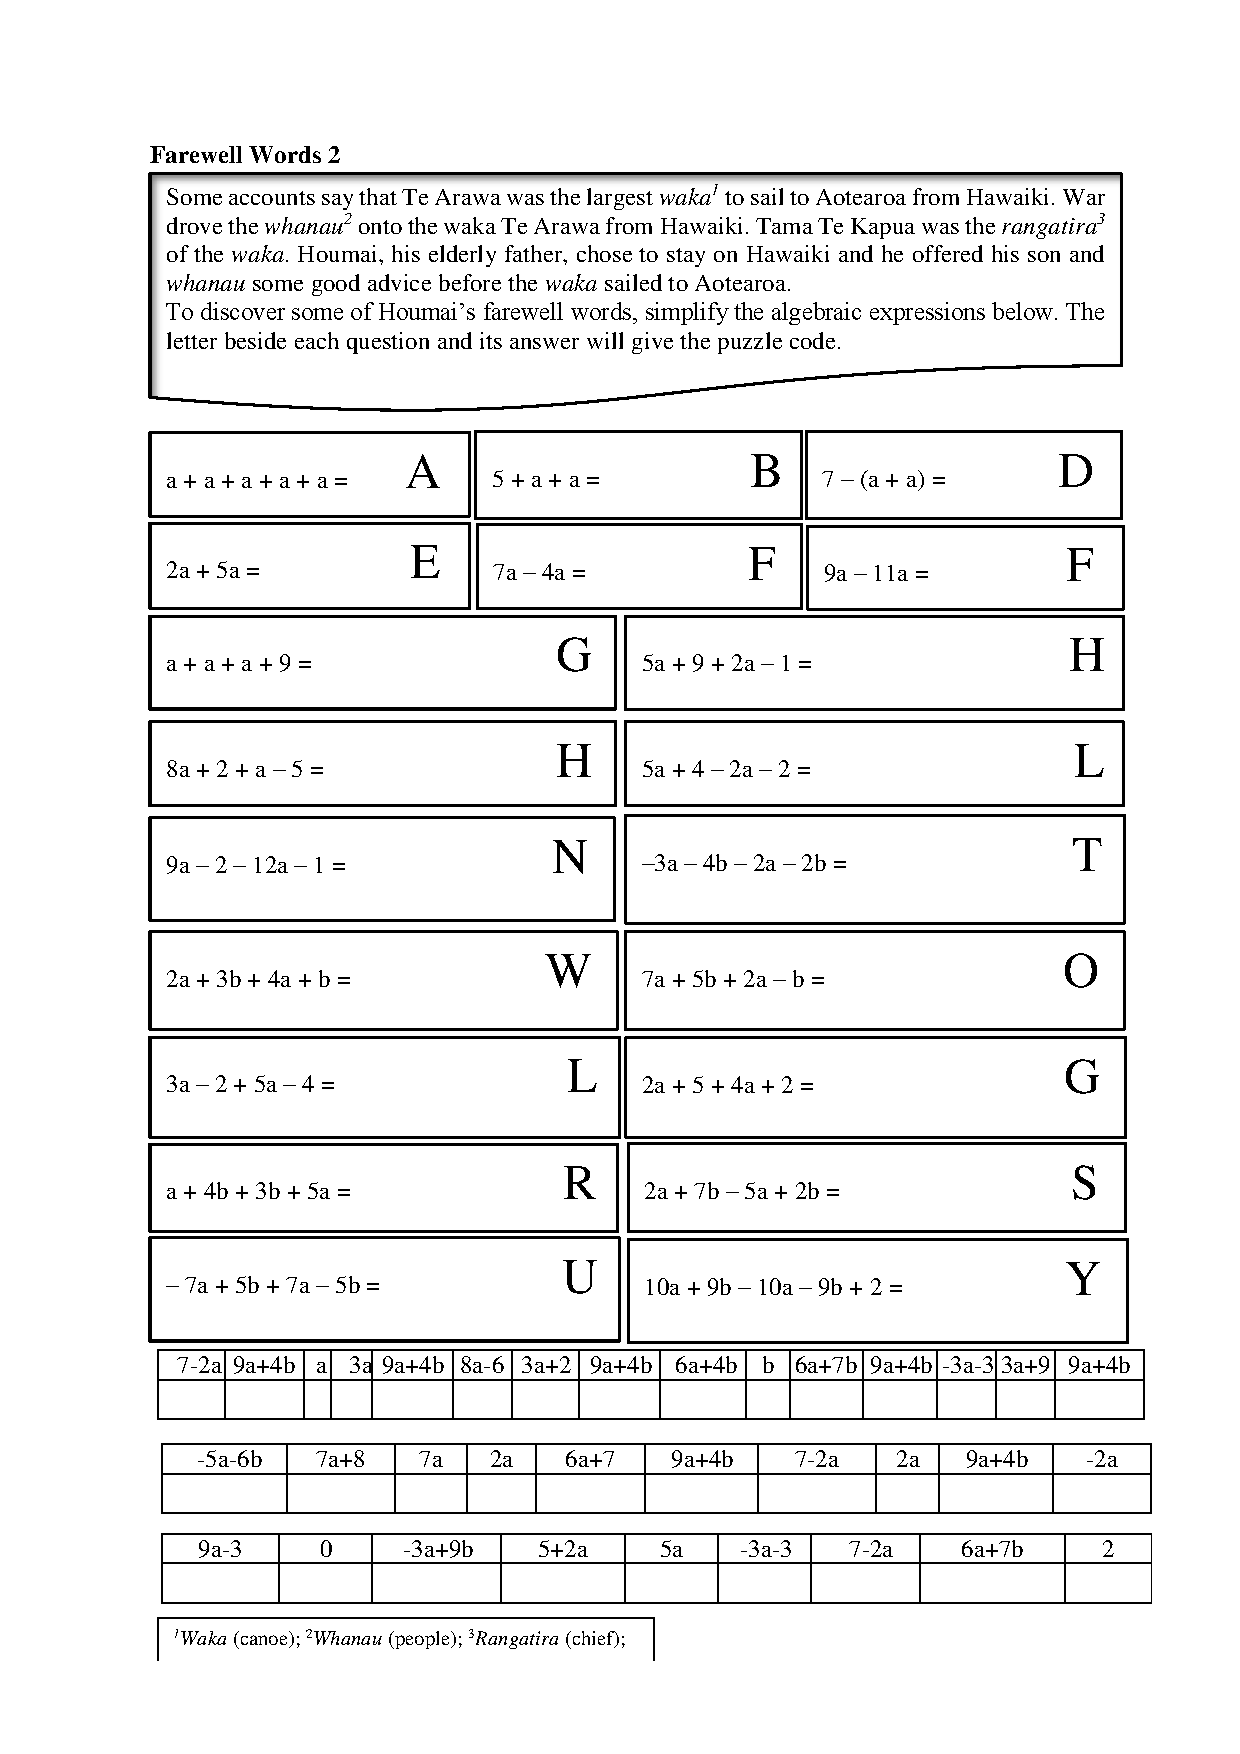
\includegraphics[width=17cm]{Qartu/Q7_Expressions_3.pdf}
\end{figure}
\newpage
\section{Multiplying Terms}
\subsection{Re-ordering multiplication}
If we have the multiplication $2 \times 5 \times 3 \times 2 \times 3 \times 2 \times 3$ we can re-order the multiplication \\
because multiplication is commutative.\\
So we can re-order the multiplication into groups of the same numbers: $2 \times 2 \times 2 \times 3 \times 3 \times 5$\\
\textbf{For the questions below:}
\begin{itemize}
	\item re-order the multiplication into groups
	\item then evaluate \underline{each} group
	\item then (use a calculator if you like) work out the value
\end{itemize}
For example: re order and calculate : $7 \times 2 \times 3 \times 3 \times 2 \times 7 \times 2$ 
\begin{align*}
&=  2 \times 2 \times 2 \times 3 \times 3 \times 7 \times 7\\
&=  8 \times 9\times 49\\
&= 3528
\end{align*}
\question
Re-order and calculate the following:
\begin{multicols}{2}
\begin{enumerate}[label=\normalsize \alph*)~~~]
	\item $5 \times 2 \times 5 \times 3 \times 5$
		\item $7 \times 2 \times 2 \times 5 \times 7$
			\item $5 \times 11 \times 2 \times 11 \times 2$
			\item $13 \times 11 \times 2 \times 13 \times 11 \times 11 \times 2$
\end{enumerate}
\end{multicols}
\questionend
\subsection{Multiplication and powers}
We can write $3 \times 3$ as $3^2$ (three to the power of 2), or $2\times 2 \times 2 \times 2$ as $2^4$ (two to the power of four).\\
\textbf{For the questions below:}
\begin{itemize}
	\item re-order the multiplications and then 
	\item write the expressions as multiplications of powers.
\end{itemize}
For example $2 \times 3 \times 5 \times 2 \times 2 \times 5 \times 2$
\begin{align*}
&=  2 \times 2 \times 2 \times 2 \times 3 \times 5 \times 5\\
&=  2^3 \times 3^1 \times 5^2\\
&= 600
\end{align*}
\newpage
\question
Write these as multiplications of powers , then calculate the answer:
\begin{multicols}{2}
\begin{enumerate}[label=\normalsize \alph*)~~~]
	\item $2 \times 5 \times 2 \times 2 \times 5 \times 2 $
	\item $7 \times 7 \times 7 \times 5 \times 2 \times 7 \times 5 $
	\item $3 \times 2 \times 3 \times 3 \times 5 \times 2  $
	\item $7 \times 3 \times 5 \times 3 \times 3 \times 3 \times 7 $
\end{enumerate}
\end{multicols}
\questionend

\subsection{Multiplying with algebra}
We can now apply the same ideas when using algebra:\\\\
For example: $b \times a \times 3 \times a \times 5 \times a$
\begin{align*}
&= 3 \times 5 \times a \times a \times a \times b\\
& = 15 \times a^3 \times b\\
& = 15a^3b
\end{align*}
\question
Re-order and simplify the following expressions:
\begin{multicols}{2}
	\begin{enumerate}[label=\normalsize \alph*)~~~]
		\item $2 \times x \times 3 \times y \times x$
		\item $5 \times x \times 4 \times x$
		\item $7 \times y \times 2 \times x \times x$
		\item $3x \times 5x \times 2$
		\item $6x \times 2x \times y$
		\item $2 \times 5x \times 3y $
		\item $3x^2 \times 2y^3$
	\end{enumerate}
\end{multicols}
\questionend
\newpage
\subsection{Adding Powers}
We can note now that :\\\\
$a^2 = a \times a$\\
and\\
$a^3 = a \times a \times a$\\\\
So: ~ $a^2 \times a^3 = \underline{a \times a } \times \underline{a \times a \times a} = a^5 $   ( so the powers get \underline{added} )\\
\question
Simplify the following:
\begin{multicols}{2}
	\begin{enumerate}[label=\normalsize \alph*)~~~]
		\item $x^2 \times x$
		\item $x \times x^3$
		\item $y^2 \times y^3 \times x$
		\item $x^2 \times y \times x^2 \times y$
		\item $6x \times 2x \times y$
		\item $2 \times 5x \times 3y \times x $
		\item $3x^2 \times 2y^3$
		\item $3x^2 \times 2y^3 \times 5 \times y$
	\end{enumerate}
\end{multicols}
\questionend \vspace{-1cm}
\newpage
\subsection{Extension: powers of terms in brackets}
\question
Work out the following powers (these will help you later on)
\begin{multicols}{3}
	\begin{enumerate}[label= \normalsize\alph*)~~~]
		\item $2^2$
		\item $2^3$
		\item $2^4$
		\item $2^5$
		\item $3^2$
		\item $3^3$
		\item $3^4$
		\item $4^2$
		\item $4^3$
		\item $5^2$
		\item $5^3$
		\item $6^2$
	\end{enumerate}
\end{multicols}
\questionend
Example:
\begin{align*}
(5a^3)^2 &= 5a^3 \times 5a^3\\
&= 5 \times 5 \times a^3 \times a^3\\
&=25a^6
\end{align*}
\question
Write these expressions without any brackets:
\begin{multicols}{2}
	\begin{enumerate}[label=\normalsize \alph*)~~~]
		\item $(3a)^2$
		\item $(5x)^2$
		\item $(2a)^3$
		\item $(4a^2)^3$
		\item $(a^2b)^3$
		\item $ (3ab^3)^2$
	\end{enumerate}
\end{multicols}
\questionend

\newpage
\quiz
\begin{figure}[!h]
	\centering
	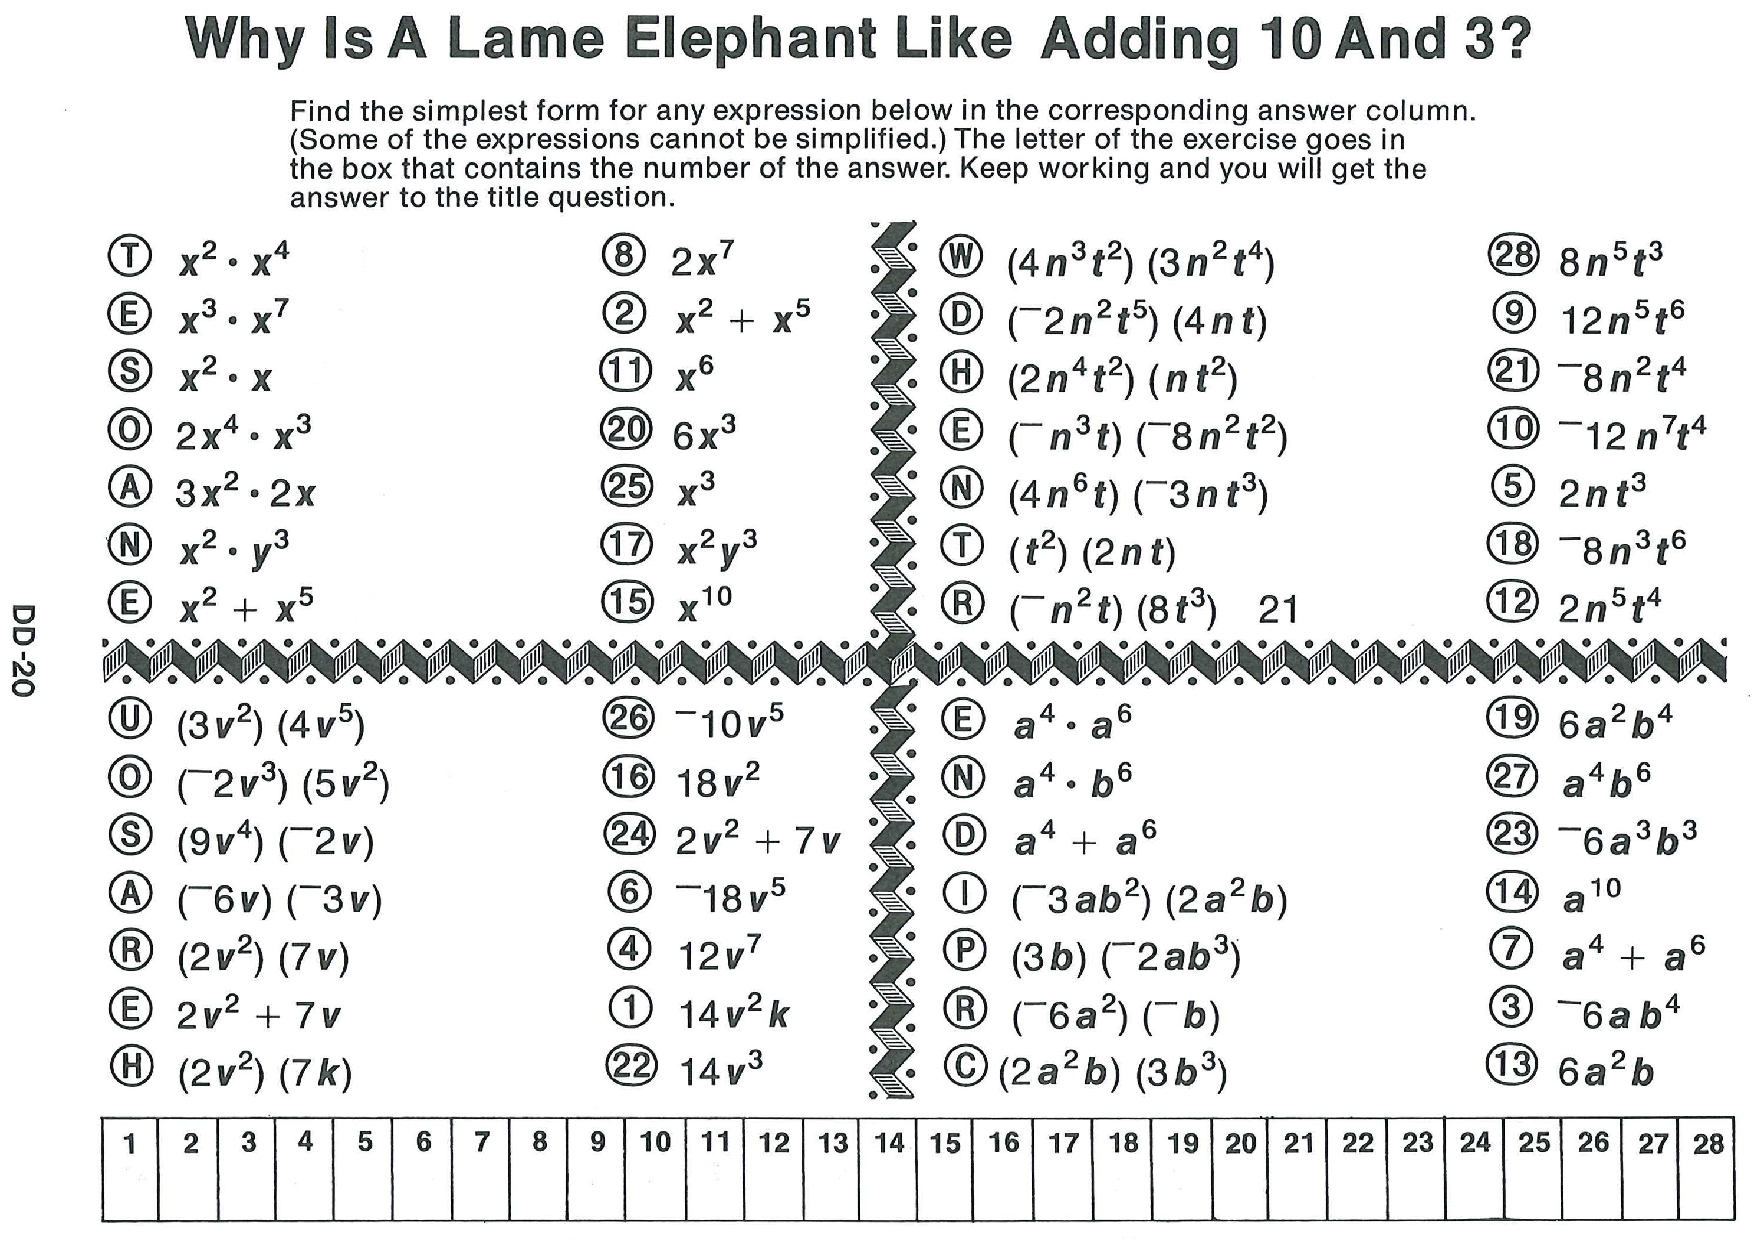
\includegraphics[height=17cm, angle=90, origin=c]{pizzazz/pizzazz_set1_7.pdf}
\end{figure}
\newpage
\quiz
\begin{figure}[!h]
	\centering
	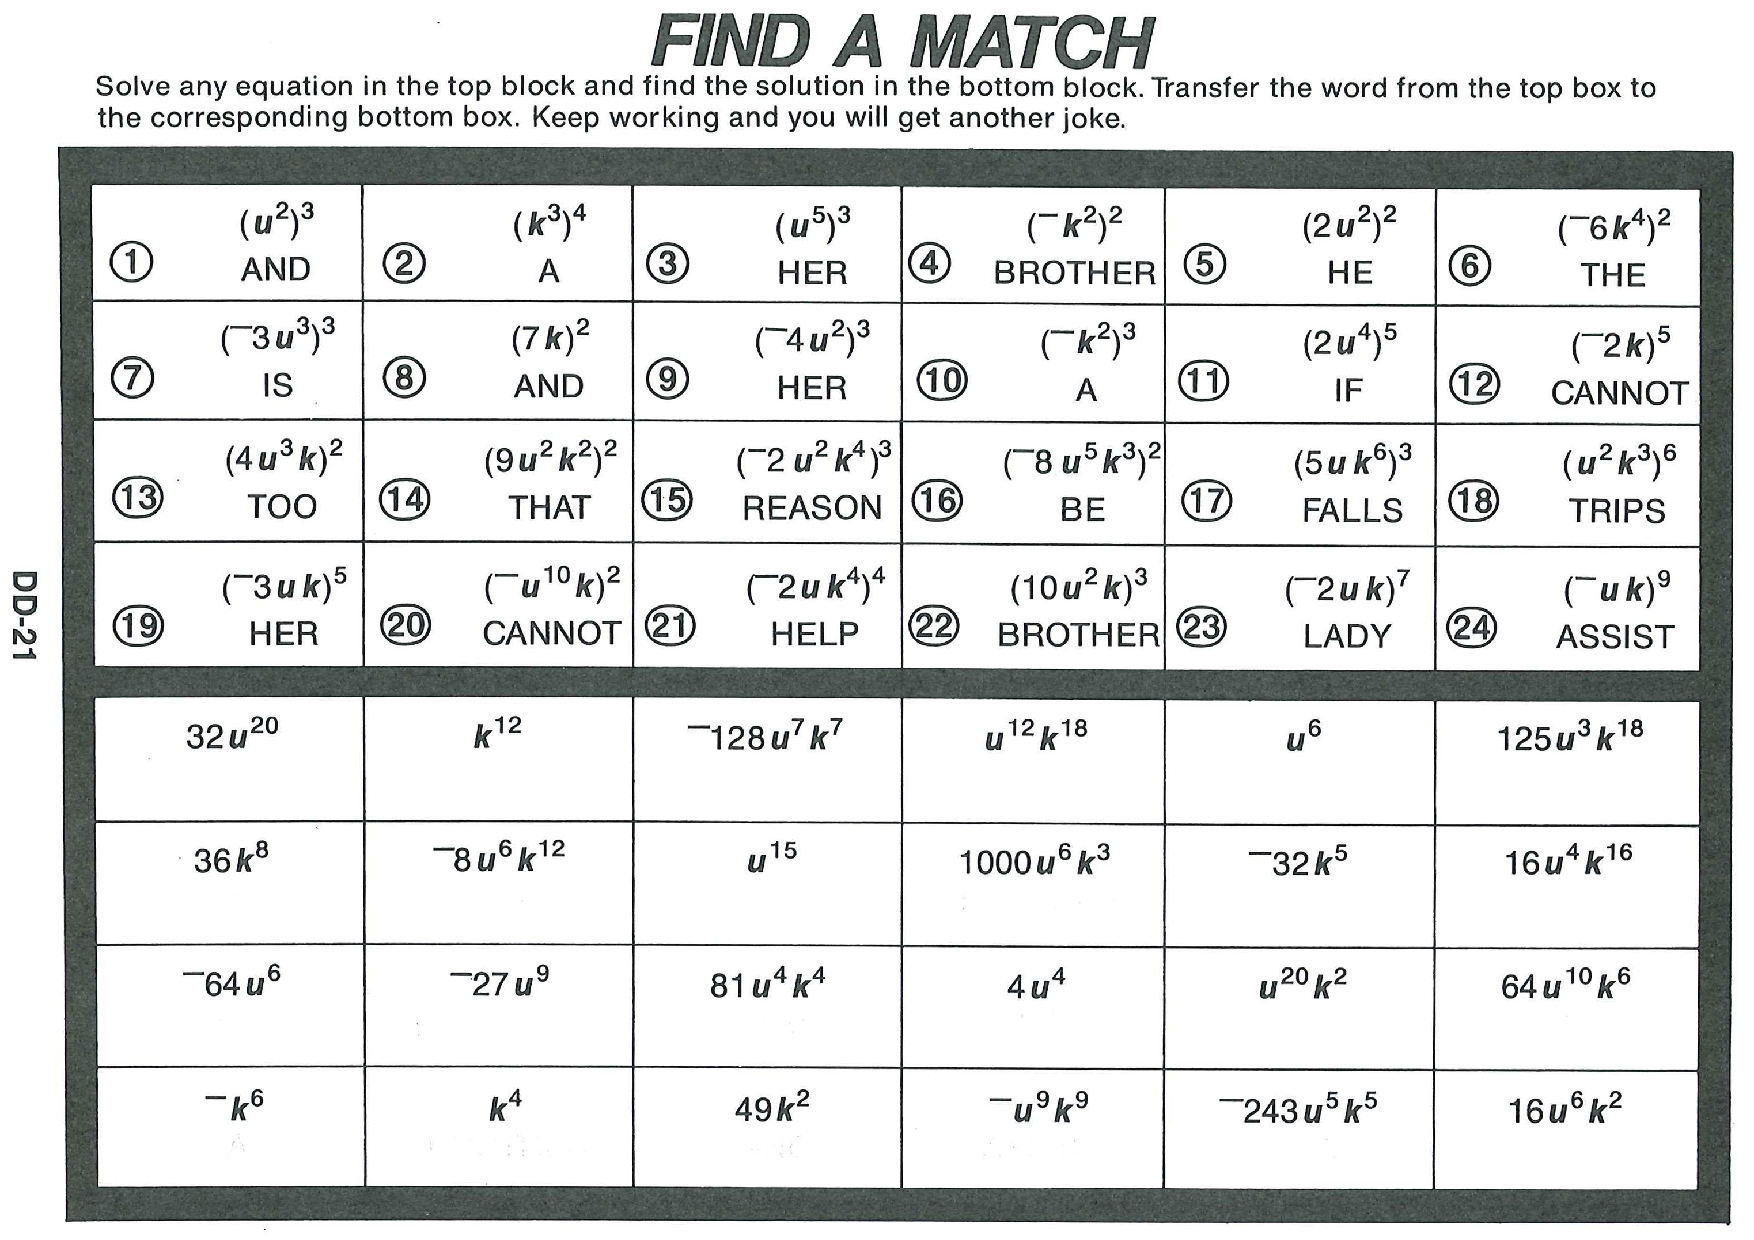
\includegraphics[height=17cm, angle=90, origin=c]{pizzazz/pizzazz_set1_1.pdf}
\end{figure}
\newpage

\section{Dividing Terms}
\subsection{Cancelling with numbers}
If we have a fraction and the numerator and denominator terms are all being multiplied,
we can cancel terms (one for one) that appear on both the numerator and the denominator:\\
For example:
\begin{align*}
\frac{2\times 3 \times 4}{3\times 4}=\frac{2 \times \cancel{3} \times \cancel{4}}{\cancel{3}\times \cancel{4}}= \frac{4}{1} = 4
\end{align*}

This is what we are doing when we are simplifying fractions:
\begin{align*}
\frac{20}{15} = \frac{4 \times 5}{ 3 \times 5 } = \frac{4 \times \cancel{5} }{ 3 \times \cancel{5} } = \frac{4}{3}
\end{align*}
\question
Simplify these fractions:
\begin{multicols}{3}
	\begin{enumerate}[label=\normalsize \alph*)~~~ , topsep=8pt,itemsep=25pt,partopsep=4pt, parsep=4pt]
		\item $\displaystyle \frac{20}{15}$
		\item $\displaystyle \frac{6}{2}$
		\item $\displaystyle \frac{4}{10}$
		\item $\displaystyle \frac{2}{8}$
		\item $\displaystyle \frac{30}{20}$
		\item $\displaystyle \frac{16}{6}$
	\end{enumerate}
\end{multicols}
\questionend \vspace{-1cm}
\subsection{Cancelling with algebra}
We can do the same thing with algebra as well
\begin{align*}
\frac{x^5}{x^2} &= \frac{x^2 \times x^3 }{x^2}\\
&=  \frac{\cancel{x^2} \times x^3 }{ \cancel{x^2} }\\
&=  \frac{x^3 }{ 1 } = x^3
\end{align*}
\question
Simplify these (algebraic) fractions:
\begin{multicols}{3}
	\begin{enumerate}[label=\normalsize \alph*)~~~ , topsep=8pt,itemsep=25pt,partopsep=4pt, parsep=4pt]
		\item $\displaystyle \frac{x^4}{x^3}$
		\item $\displaystyle \frac{y}{y^2}$
		\item $\displaystyle \frac{xy}{x^2y}$
		\item $\displaystyle \frac{a^3}{ab^2}$
		\item $\displaystyle \frac{b^2}{b}$
		\item $\displaystyle \frac{b^2}{b^3}$
	\end{enumerate}
\end{multicols}
\questionend

\subsection{Bringing it together}
We can now combine this to simplify fractions that contain both numbers and letters.
Simplify:
\begin{align*}
\frac{12x^3y}{16x^2y}&= \frac{3 \times 4 \times x \times x^2 \times y }{4 \times 4 \times x^2 \times y}\\
                                     &= \frac{3 \times \cancel{4} \times x \times \cancel{x^2}  \times \cancel{y}  }{4 \times \cancel{4}  \times \cancel{x^2} \times \cancel{y} }\\
                                     & =  \frac{3  \times x    }{4   \times 1 }\\
                                     &= \frac{3x}{4}
\end{align*}
\question
Simplify these fractions:
\begin{multicols}{3}
	\begin{enumerate}[label=\normalsize \alph*)~~~ , topsep=8pt,itemsep=25pt,partopsep=4pt, parsep=4pt]
		\item $\displaystyle \frac{20x^4}{15x^3}$
		\item $\displaystyle \frac{6y}{2y^2}$
		\item $\displaystyle \frac{4xy}{10x^2y}$
		\item $\displaystyle \frac{2a^3}{8ab^2}$
		\item $\displaystyle \frac{30b^2}{20b}$
		\item $\displaystyle \frac{16b^2}{6b^3}$
	\end{enumerate}
\end{multicols}
\questionend
\question
Simplify the fraction and the evaluate using the substitution given:
\begin{multicols}{2}
	\begin{enumerate}[label=\normalsize \alph*)~~~ , topsep=8pt,itemsep=25pt,partopsep=4pt, parsep=4pt]
\item For $\displaystyle A = \frac{3b^2}{2b}$ , find $A$ if $b=4$
\item For $\displaystyle B = \frac{18c^5}{12c^3}$ , find $B$ if $c=5$
\item For $\displaystyle C = \frac{24d}{36d^3}$ , find $C$ if $d=2$
\item For $\displaystyle D = \frac{18e^2f}{12ef^2}$ , find $D$ if $e=1, f=-1$
\item For $\displaystyle G = \frac{27hj}{18h^2}$ , find $D$ if $h=5, j=2$
\item For $\displaystyle K = \frac{28l^2m^9}{26l^3m^5}$ , find $K$ if $l=7, m=2$
	\end{enumerate}
\end{multicols}
\questionend

\newpage
\quiz
\begin{figure}[!h]
	\centering
	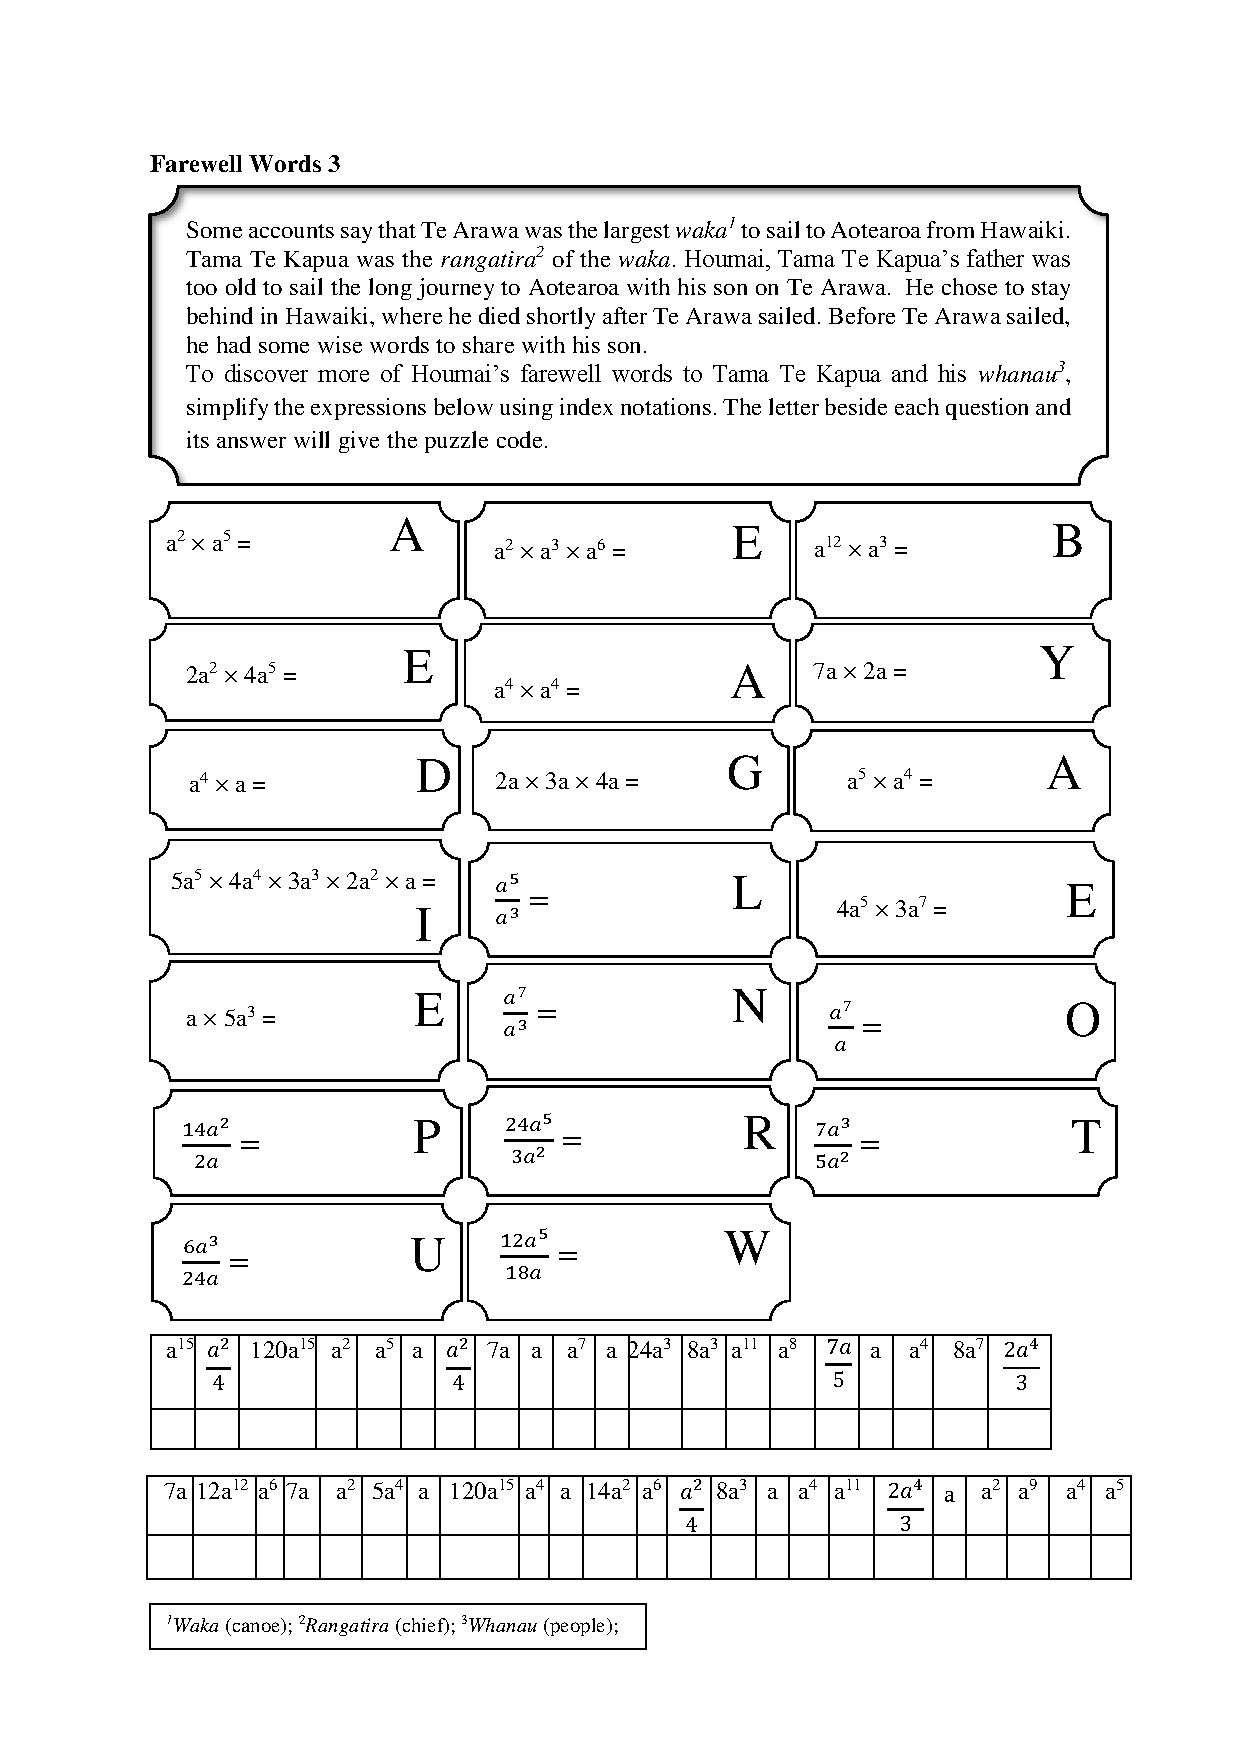
\includegraphics[width=16cm]{Qartu/Q7_Expressions_4.pdf}
\end{figure}
\newpage
\quiz
\begin{figure}[!h]
	\centering
	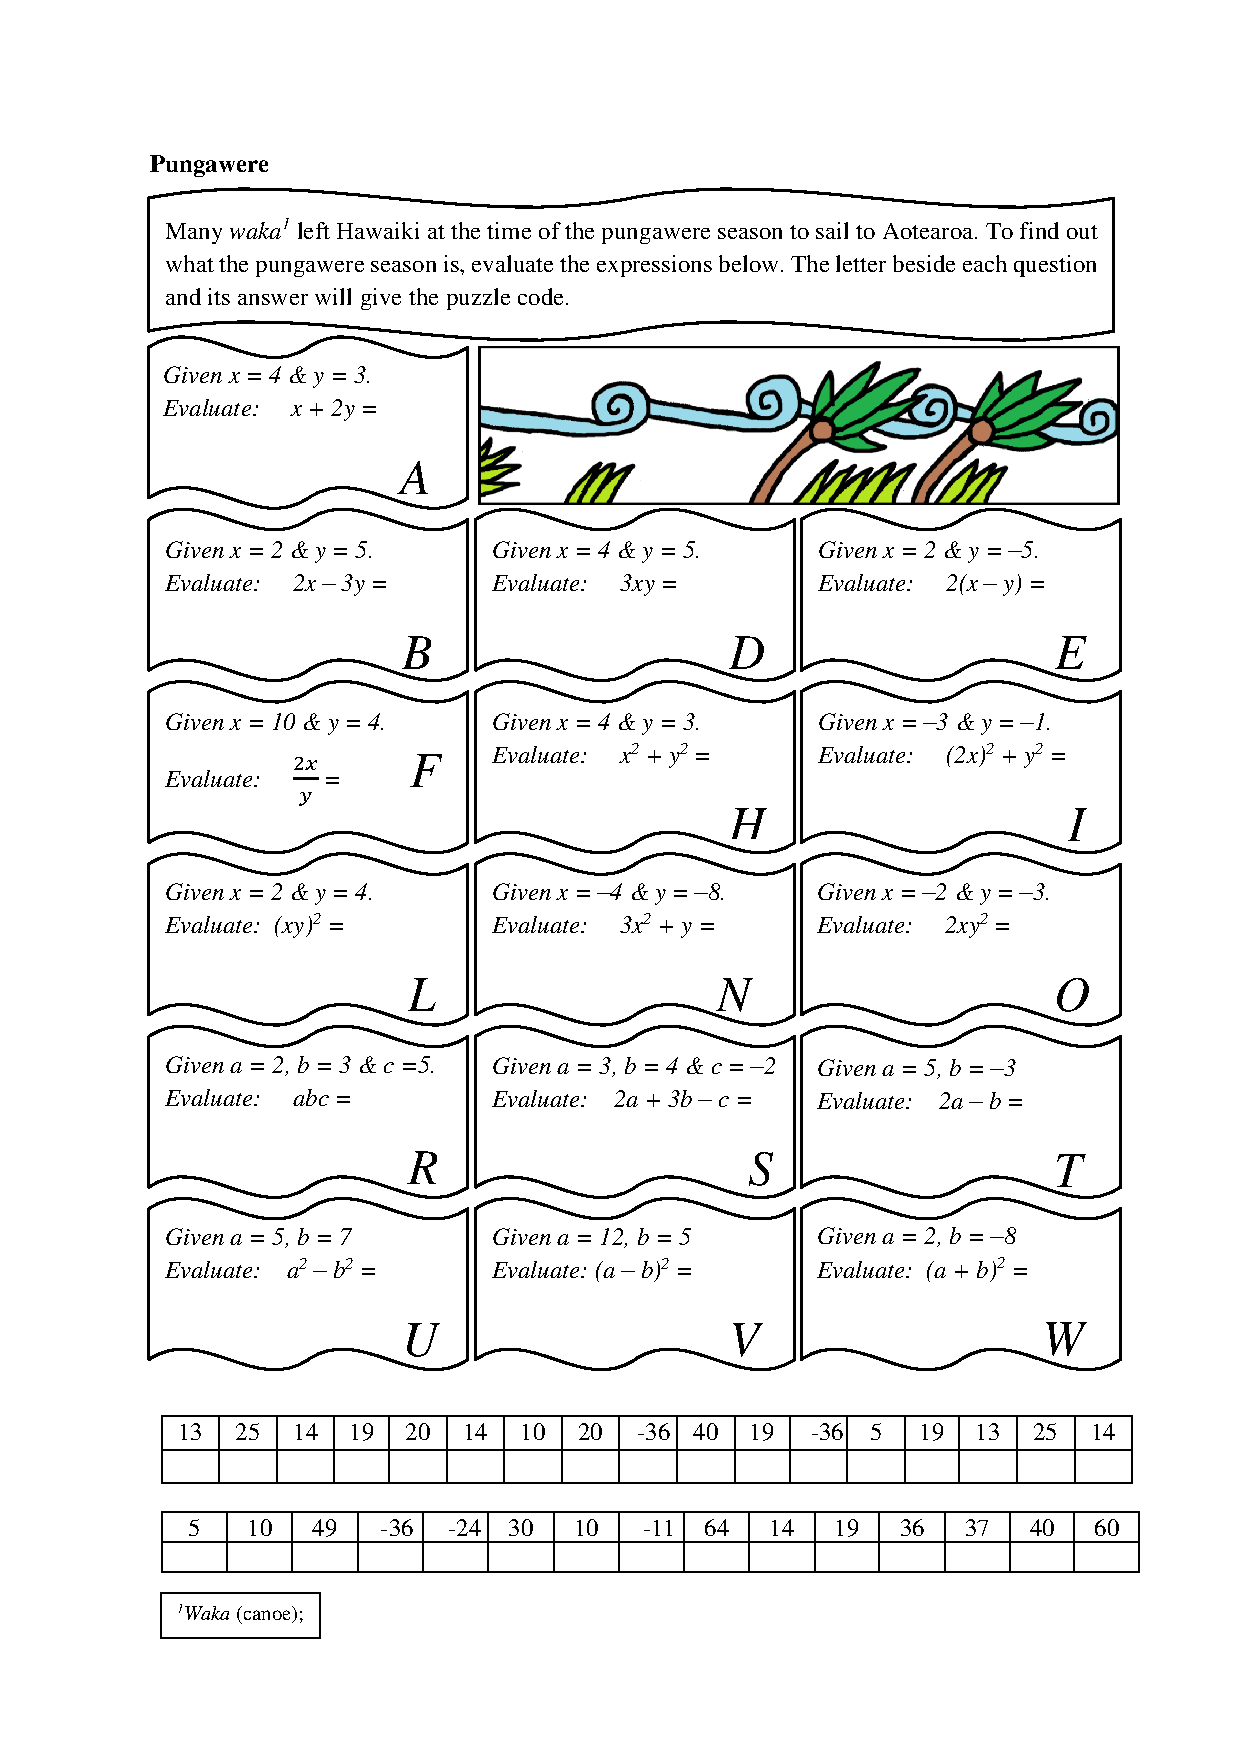
\includegraphics[width=16cm]{Qartu/Q7_Expressions_7.pdf}
\end{figure}
\newpage
\section{Multiplying Algebraic Fractions}
When we \textbf{multiply} fractions, we multiply the numerators and multiply the denominators:
\setlength{\columnsep}{-6cm}
\begin{multicols}{2}
	~\vspace{-1cm}
\begin{align*}
\frac{4}{5} \times \frac{2}{3}&= \frac{4 \times 2}{5 \times 3}\\
&=  \frac{8}{15} \\
\end{align*}
\begin{align*}
\frac{2}{3} \times \frac{1}{2}&= \frac{2 \times 1}{3 \times 2}\\
&=  \frac{\cancel{2} \times 1}{3 \times \cancel{2} } \\
& =  \frac{1   }{3}\\
\end{align*}
\end{multicols}\vspace{-1cm}
\setlength{\columnsep}{1cm}
\question
Multiply and , where necessary, simplify these fractions:\\
\begin{multicols}{3}
	\begin{enumerate}[label=\normalsize \alph*)~~~ , topsep=8pt,itemsep=25pt,partopsep=4pt, parsep=4pt]
		\item $\displaystyle \frac{1}{2} \times \frac{1}{4}$
		\item $\displaystyle  \frac{3}{4} \times \frac{1}{3}$
		\item $\displaystyle \frac{1}{12} \times \frac{6}{1}$
		\item $\displaystyle \frac{7}{9} \times \frac{3}{5}$
		\item $\displaystyle \frac{3}{8} \times \frac{1}{4}$
		\item$\displaystyle \frac{2}{9} \times \frac{1}{2}$
	\end{enumerate}
\end{multicols}\vspace{0.5cm}
\questionend
Similarly for algebra
\setlength{\columnsep}{-4cm}
\begin{multicols}{2}
	~\vspace{-1cm}
	\begin{align*}
		\frac{2a}{b} \times \frac{a^2}{b}&= \frac{2a \times a^2}{b \times b}\\
		&=  \frac{2a^3}{b^2} \\
	\end{align*}
	\begin{align*}
		\frac{3a^2}{2b} \times \frac{ab^2}{a^2}&= \frac{3a^2  \times ab^2 }{2b \times a^3}\\
		&= \frac{3a^3b^2 }{2a^3b}\\
		& = \frac{3 }{2} \times \frac{\cancel{a^2} }{ \cancel{a^2} } \times \frac{b \times \cancel{b} }{\cancel{b}}\\
		& = \frac{3b}{2}
	\end{align*}
\end{multicols}
\setlength{\columnsep}{1cm}
\question
Multiply and , where necessary, simplify these algebra fractions:\\
\begin{multicols}{3}
	\begin{enumerate}[label=\normalsize \alph*)~~~ , topsep=8pt,itemsep=25pt,partopsep=4pt, parsep=4pt]
		\item $\displaystyle \frac{3a^2}{4} \times \frac{1}{b}$
		\item $\displaystyle  \frac{2b^2}{a} \times \frac{b}{3}$
		\item $\displaystyle \frac{12a}{b^2} \times \frac{a^3}{4b}$
		\item $\displaystyle \frac{4a}{6b} \times \frac{a^3}{2b^2}$
		\item $\displaystyle \frac{12a^2}{b^2} \times \frac{b}{2a^2}$
		\item$\displaystyle \frac{4ab}{3} \times \frac{2a}{b^2}$
	\end{enumerate}
\end{multicols}\vspace{0.5cm}
\questionend


\newpage
\section{Adding Algebraic Fractions}
The lowest common multiple of $4, 6$ is $12$,\\ because $12$ is a multiple of $4$ and $12$ is a multiple of $3$, and it is the first number where this is the case.
\question
 Find the lowest common multiple of the pair of numbers given below:
\begin{multicols}{3}
	\begin{enumerate}[label=\normalsize \alph*)~~~ , topsep=8pt,itemsep=25pt,partopsep=4pt, parsep=4pt]
		\item $2, 3$
		\item $4,5$
		\item $6,8$
		\item $5,15$
		\item $4, 10$
		\item $6,9$
	\end{enumerate}
\end{multicols}\vspace{0cm}
\questionend
\question
Find these equivalent fractions:
\begin{multicols}{3}
	\begin{enumerate}[label=\normalsize \alph*)~~~ , topsep=8pt,itemsep=25pt,partopsep=4pt, parsep=4pt]
		\item $\displaystyle \frac{x}{3}=\frac{\square}{6}$
		\item $\displaystyle \frac{y}{2}=\frac{\square}{6}$
		\item $\displaystyle \frac{3x}{5}=\frac{\square}{20}$
		\item $\displaystyle \frac{2y}{4}=\frac{\square}{20}$
		\item $\displaystyle \frac{3x}{5}=\frac{\square}{35}$
		\item $\displaystyle \frac{2y}{7}=\frac{\square}{35}$
	\end{enumerate}
\end{multicols}\vspace{0cm}
\questionend
\question
Add these fractions:
\begin{multicols}{3}
	\begin{enumerate}[label=\normalsize \alph*)~~~ , topsep=16pt,itemsep=25pt,partopsep=4pt, parsep=4pt]
		\item $\displaystyle \frac{x}{3} + \frac{x}{2}\\\\ =\frac{\square}{6}+\frac{\square}{6}\\\\ =\frac{\square}{6}$
		\item $\displaystyle \frac{3x}{5} - \frac{2x}{4}\\\\=\frac{\square}{20} - \frac{\square}{20}\\\\ = \frac{\square }{20}$
		\item $\displaystyle \frac{3y}{5} - \frac{2y}{7}\\\\=\frac{\square}{35} - \frac{\square}{35} \\\\ = \frac{\square}{35}$
	\end{enumerate}
\end{multicols}
\questionend
\newpage
\question
 Add these fractions:
\begin{multicols}{3}
\begin{enumerate}[label=\normalsize \alph*)~~~ , topsep=16pt,itemsep=25pt,partopsep=4pt, parsep=4pt]
\item $\displaystyle \frac{x}{3} + \frac{y}{2}\\\\ =\frac{\square}{6}+\frac{\square}{6}\\\\ =\frac{\square + \square }{6}$
\item $\displaystyle \frac{3x}{5} - \frac{2y}{4}\\\\=\frac{\square}{20} - \frac{\square}{20}\\\\ = \frac{\square  - \square }{20}$
\item $\displaystyle \frac{3x}{5} + \frac{2y}{7}\\\\=\frac{\square}{35} + \frac{\square}{35} \\\\ = \frac{\square + \square }{35}$
	\end{enumerate}
\end{multicols}
\questionend
\question
 Add these fractions:
\begin{multicols}{3}
\begin{enumerate}[label=\normalsize \alph*)~~~ , topsep=16pt,itemsep=25pt,partopsep=4pt, parsep=4pt]
	\item $\displaystyle \frac{x}{6} + \frac{x}{4}$
	\item $\displaystyle \frac{-8x}{3} + \frac{2x}{7}$
	\item $\displaystyle \frac{11y}{2} - \frac{y}{8}$
	\item $\displaystyle \frac{x}{3} + \frac{x}{2}$
	\item $\displaystyle \frac{-3x}{5} - \frac{2x}{4}$
	\item $\displaystyle \frac{-3y}{5} - \frac{-2y}{7}$
\end{enumerate}
\end{multicols}
\questionend
\question
 Add these fractions:
\begin{multicols}{3}
	\begin{enumerate}[label=\normalsize \alph*)~~~ , topsep=16pt,itemsep=25pt,partopsep=4pt, parsep=4pt]
		\item $\displaystyle \frac{x}{5} + \frac{y}{2}$
		\item $\displaystyle \frac{3y}{2} - \frac{8x}{3}$
		\item $\displaystyle \frac{3x}{5} + \frac{2y}{7}$
		\item $\displaystyle \frac{x}{5} + \frac{y}{2}+\frac{x}{1}$
		\item $\displaystyle \frac{3y}{2} - \frac{8x}{3}-\frac{x}{2}$
		\item $\displaystyle \frac{-3x}{5} - \frac{2y}{7} - \frac{-5y}{7}$
	\end{enumerate}
\end{multicols}
\questionend
\newpage
\section{Linear Equations}
\subsection{Basic Linear Equations}
Examples:
\renewcommand{\tabcolsep}{16pt}
\renewcommand{\arraystretch}{2}
\begin{center}
\begin{tabular}{ p{6cm} | p{6cm} }\hline
Solve: $x+8 = 4$ & Solve: $\displaystyle \frac{x}{5}=3$ \\
$\begin{aligned}[t] % placement: default is "center", options are "top" and "bottom"
x + 8 &= 4 &\\
x + 8 - 8 &= 4 - 8 &\text{~~~~~~~~~}(-8)\\
x &= -4 &\text{~~~~~~~~~}\\
\end{aligned}$
& 
$\begin{aligned}[t] % placement: default is "center", options are "top" and "bottom"
\frac{x}{5} &= 3 &\\
\frac{x}{5} \times 5 &= 3 \times 5 &\text{~~~~~~~~~}(\times 3)\\
x &= 15 &\text{~~~~~~~~~}\\
\end{aligned}$
\\\hline
Solve: $x-5= 9$ & Solve: $\displaystyle 6x=48$ \\
$\begin{aligned}[t] % placement: default is "center", options are "top" and "bottom"
x - 5 &= 9 &\\
x - 5 + 5 &= 9 + 5 &\text{~~~~~~~~~}(+5)\\
x &= 14 &\text{~~~~~~~~~}\\
\end{aligned}$
& 
$\begin{aligned}[t] % placement: default is "center", options are "top" and "bottom"
6x&=48 &\\
\frac{6x}{6} &= \frac{48}{6} &\text{~~~~~~~~~}(\ / 6)\\
x &= 8 &\text{~~~~~~~~~}\\
\end{aligned}$
\\\hline
\end{tabular}
\end{center}\vspace{0.5cm}


\question
Find $x$:\\
Make sure you write at least one line of working:
\begin{multicols}{3}
\begin{enumerate}[label=\normalsize \alph*)~~~]
\item $x + 6 = 30$
\item $x - 9 = 15$
\item $x + 8 = -4$
\item $x - 15 = -33$
\item $8x = 40$
\item $-12x = -132$
\item $9x = -117$
\item $-4x = 136$
\item $\displaystyle \frac{x}{9} = -14$
\item $\displaystyle \frac{-x}{5} = 13$
\item $x-4 = 26$
\item $\displaystyle \frac{x}{8} = 13$
\item $4x - 13 = 15$
\item $-3x - 16 = 35$
\item $16 - 7x = 107$
\item $-38 + 5x = 22$
\end{enumerate}
\end{multicols}
\questionend
\newpage
\quiz
\begin{figure}[!h]
	\centering
	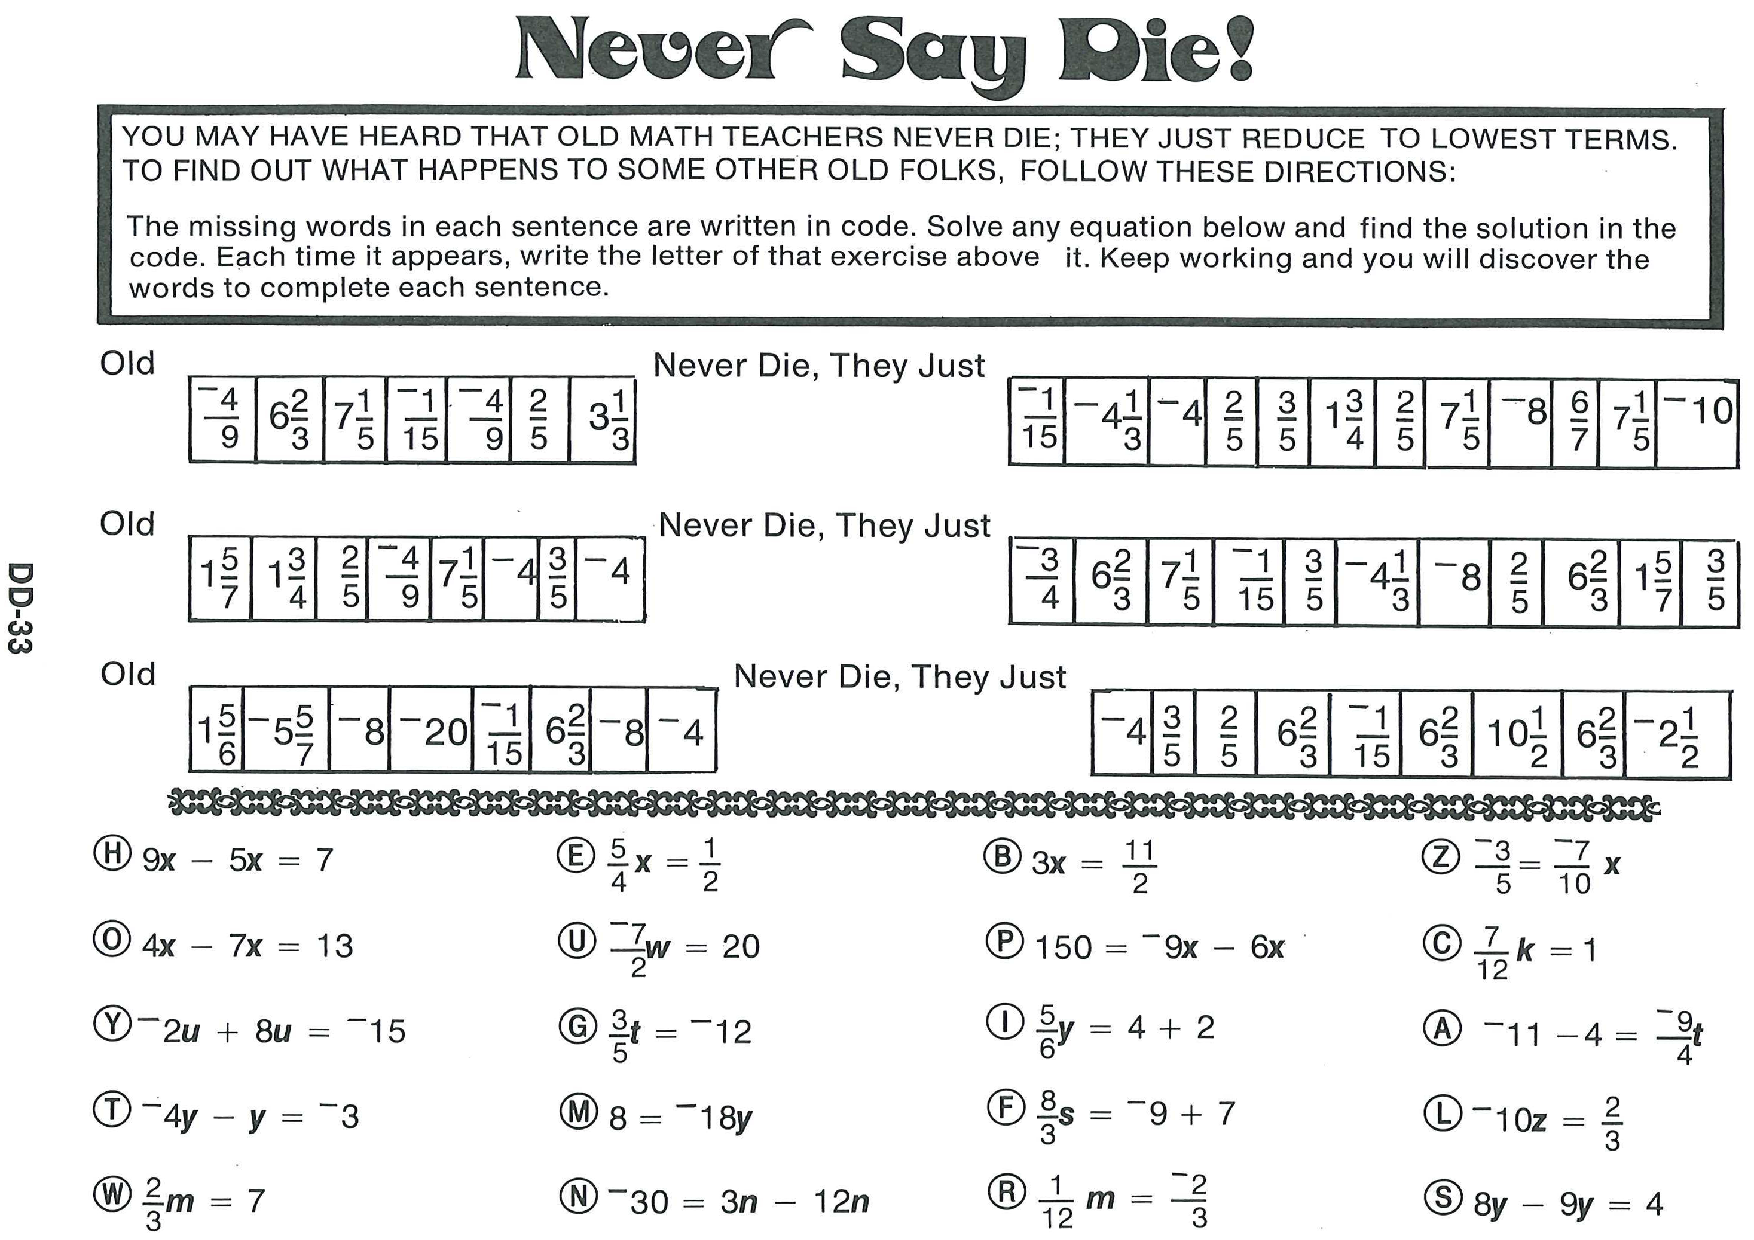
\includegraphics[height=17cm, angle=90, origin=c]{pizzazz/pizzazz_set1_5.pdf}
\end{figure}
\newpage
\subsection{Linear Equations with the unknown on both sides}
\question
Find $x$:
\begin{multicols}{2}
\begin{enumerate}[label=\normalsize \alph*)~~~]
\item $5x = 2x - 15$
\item $4x - 5 = -2x - 23$
\item $-5x + 3 = 4x - 69$
\item $-8x + 40 = -4x + 136$
\item $-5x+5 = 3x-43$
\item $-4x + 40 = 4x - 64$
\item $14x + 20 = 21x - 43$
\item $-3x -15 = - 5x + 73$
\item $6x -4 = 2x + 6$
\item $-7x - 23 = -10x - 15$
\item $3x + 12 = 7x + 9$
\item $14 - 3x = -7x - 8$
\end{enumerate}
\end{multicols}
\questionend
\newpage
\subsection{Linear Equations with Words}
\question
Form an equation involving ‘x’ for each question below and then solve it. Show your working.

\begin{enumerate}[label=\normalsize \alph*)~~~]
\item Four times a number minus seven gives the same result as two times the same number plus fifteen. \\
What is the number?
\item Jason and his friend earn the same hourly rate for a job. \\
Jason works 15 hours while his friend works 12 hours, but gets an extra payment of \$45.\\
 What is Jason’s and his work mate's hourly rate if their pay is the same for the job?
\item Tabitha can purchase seven ink cartridges from a store in town or order six cartridges online and pay a \$15 courier charge.\\
 If the cost is to be the same, what is the price of a single ink cartridge?
\item Steve and his neighbour get their cars repaired at the same garage.\\
 Steve’s account shows six hours labour and parts costing \$125.\\
 His neighbour’s account shows three hours labour and \$290 for parts.\\
 If their accounts are for the same amount, what hourly labour rate does the garage charge? 
\item The cost of hiring a motor home for seven days and paying \$800 for insurance is exactly the same as a special deal of twelve days hireage with reduced insurance of \$240. \\
What is the cost per day of hiring the motor home?
\item Two guests stay in the same hotel.\\
 Guest A stays for 12 nights and spends an additional \$490 on meals etc, while guest B stays for 6 nights and spends an additional \$844 on meals etc.\\
 If both guests end up paying the same amount for their respective stay, what is the hotels’s room rate per night?
\item Eight times a number plus eleven gives the same result as four times the same number minus thirteen. \\
What is the number?
\item A boy cycles for three hours at a certain speed and then at double that speed for the next two hours. \\
If he travels a total of 126 km altogether, what is his initial speed in km/h?
\end{enumerate}
\questionend
\newpage
\quiz
\begin{figure}[!h]
	\centering
	\includegraphics[width=17cm, angle=0, origin=c]{pizzazz/pizzazz_set1_6.pdf}
\end{figure}
\newpage
\subsection{Linear Equations with Brackets}
\quiz
\begin{figure}[!h]
	\centering
	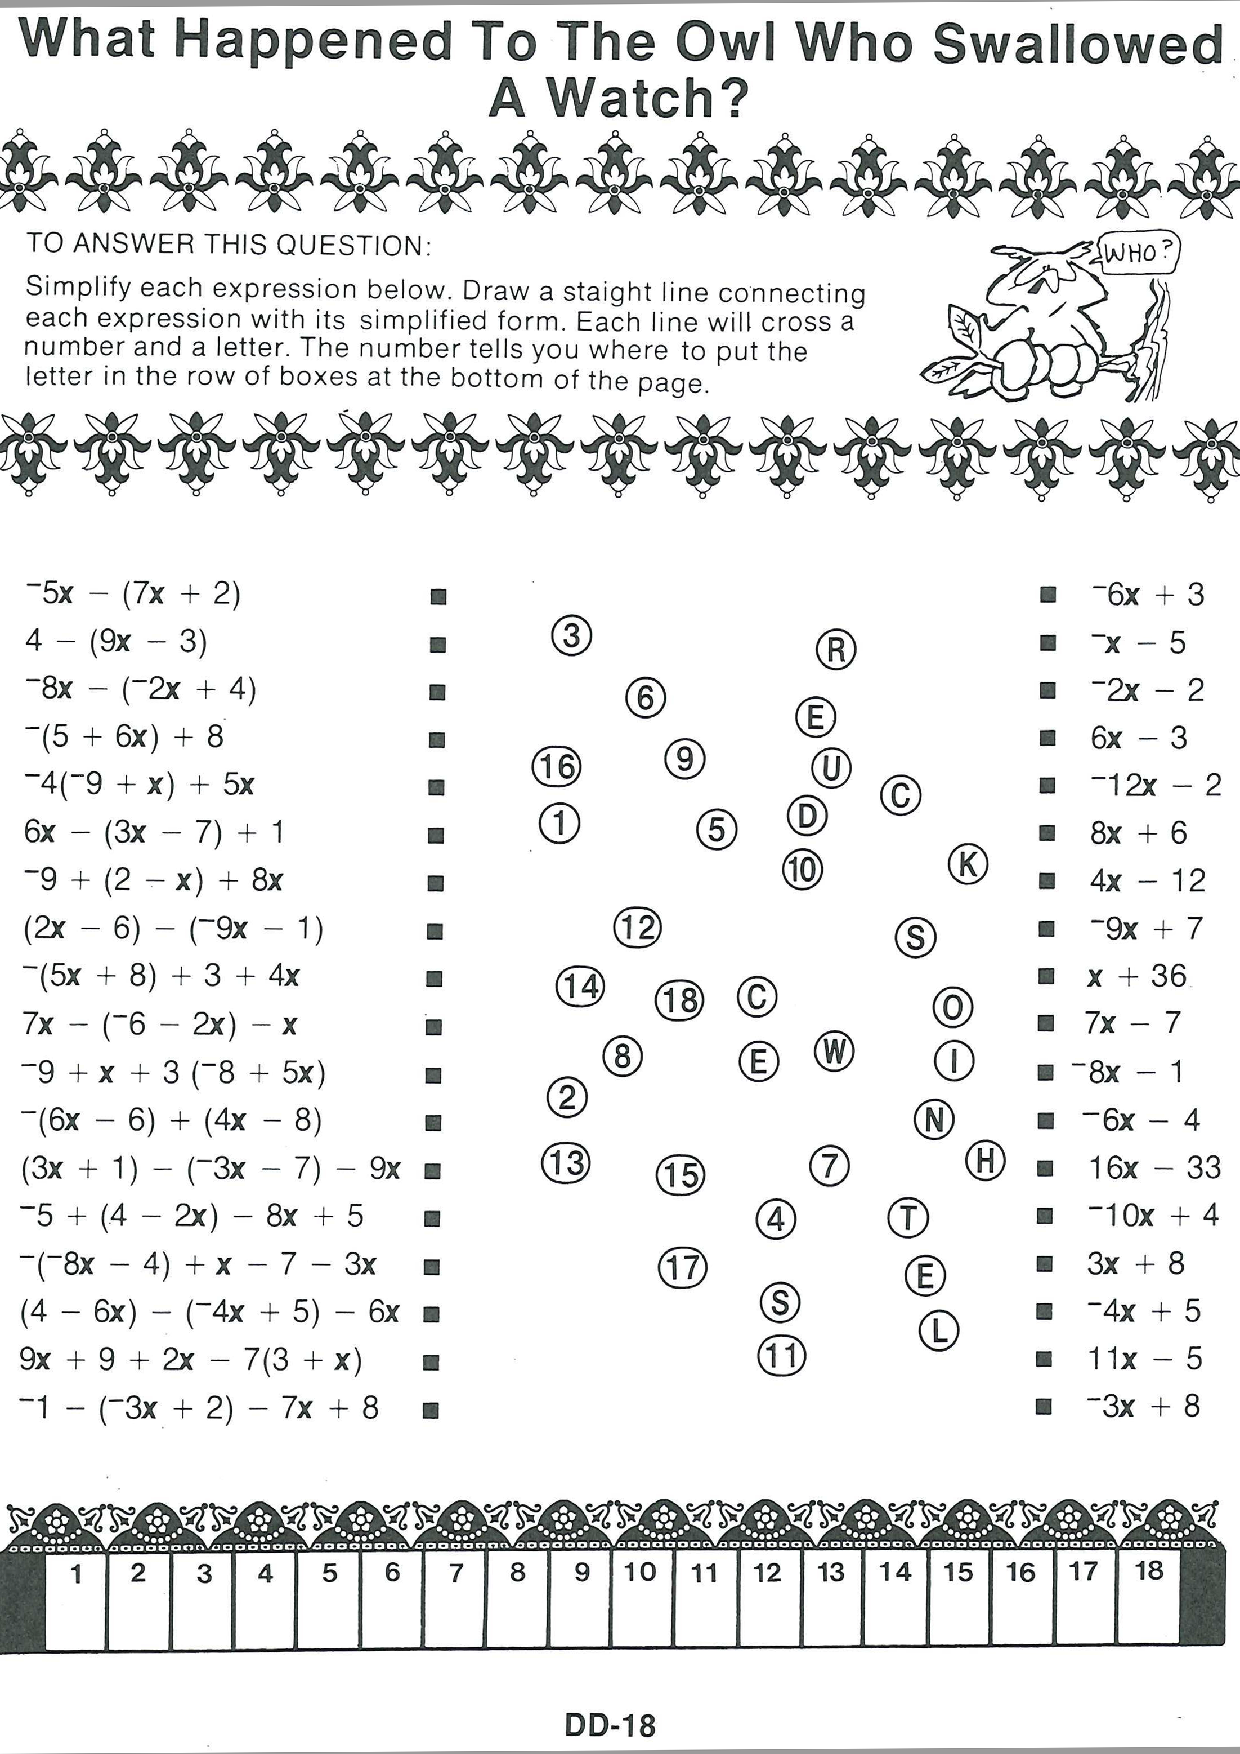
\includegraphics[width=16cm, angle=0, origin=c]{pizzazz/pizzazz_set1_8.pdf}
\end{figure}
\newpage
\question
Expand brackets and re-arrange, to find $x$ 

\begin{multicols}{2}
	\begin{enumerate}[label=\normalsize \alph*)~~~]
\item $4(x + 7) = 64$
\item $5(x - 8) = 40$
\item $7(x - 2) = -42$
\item $6(x + 4) = -54$
\item $4(3x + 1) = 76$
\item $-6(x - 1) = -61$
\item $3(7 + x) = 20$
\item $7(2x - 3) = -14$
\item $9(1 - 5x) = 324$
\item $-3(2 + 5x) = 99$
\item $2(10 - x) = 17$
\item $5(7 - 6x) = 40$
\item $3(2x + 5) + x = -20$
\item $2(1 - 4x) - 2x = 27$
\item $-4(2x - 6) + 3x = 20$
\item $2(3x + 5) - 2(x + 1) = 20$
\end{enumerate}
\end{multicols}
\questionend\vspace{-1cm}
\subsection{Linear Equations with Words}
\question
Form an equation involving ‘x’ for each question below and then solve.

	\begin{enumerate}[label=\normalsize \alph*)~~~]
\item Jake thinks of a number and adds eight to it. \\
He then multiplies his answer by four and gets 68. \\
What was his original number?
\item Taylor thinks of a number and subtracts six from it. \\
She then multiplies it by seven and gets 98. \\
What was her original number?

\item Jacob has \$19 and Peter \$33. \\
How much must Jacob give Peter so that Peter has three times as much as Jacob?
\item Find the two consecutive numbers that when the smaller is multiplied by five and the large by three the total is 75?
\item Emily’s father is 8 times as old as her. \\
In ten years’ time Emily’s father will be only three times older than her. \\
What are Emily and her father’s present ages?
\item Find the two consecutive numbers that seven times the smaller is four less than six times the greater.
\end{enumerate}
\questionend
\newpage
\quiz
\begin{figure}[!h]
	\centering
	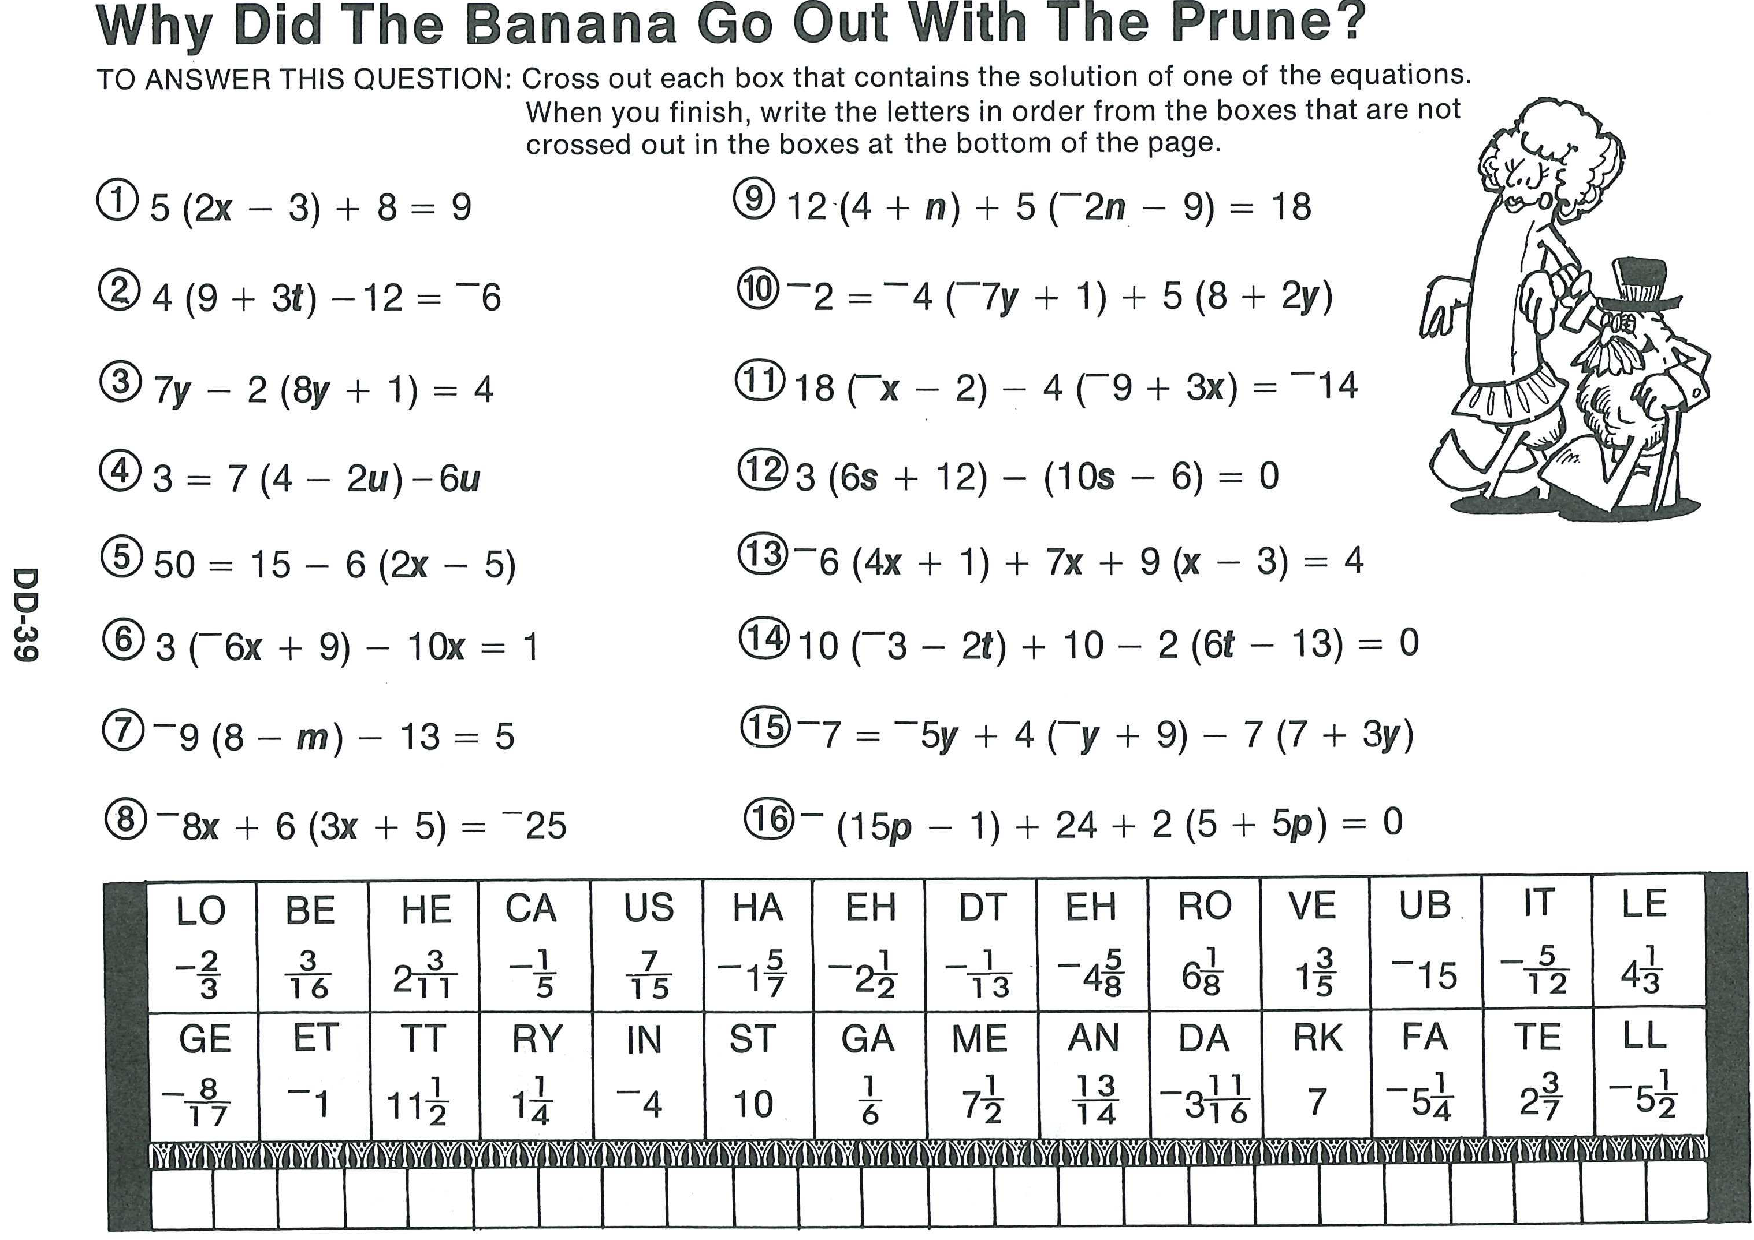
\includegraphics[height=17cm, angle=90, origin=c]{pizzazz/pizzazz_set1_9.pdf}
\end{figure}

\newpage
\subsection{Linear Equations with Fractions}
\question
Solve these equations, for $x$:
\begin{multicols}{2}
	\begin{enumerate}[label=\normalsize \alph*)~~~]
\item $\displaystyle \frac{3x+1}{7} = 4$
\item $\displaystyle  \frac{5x - 3}{4} = 8$
\item $\displaystyle  \frac{x}{3} + 14 = 2$
\item $\displaystyle \frac{2x}{3} - 12 = 40$
\item $\displaystyle \frac{x}{3} - \frac{x}{5} = 4$
\item $\displaystyle \frac{3x}{2} + \frac{x}{4} = 14$
\item $\displaystyle \frac{5x}{3} + 1 = \frac{x}{6} + 3$
\item $\displaystyle \frac{4x+3}{5} = \frac{x+3}{2}$
\item $\displaystyle \frac{x+6}{4} = \frac{x}{2}$
\item $\displaystyle 1 - x = \frac{x+6}{9}$
\end{enumerate}
\end{multicols}
\questionend\vspace{-1cm}
\newpage
\subsection{Linear Equations with Words}
\question
Form an equation involving ‘x’ for each question below and then solve. Show your working.

\begin{enumerate}[label=\normalsize \alph*)~~~]
\item Sue thinks of a number and adds 55 to it then divides the result by three.\\
 If the answer is four, what is the original number?
\item Leanne adds 42 to a number and then halves the result.\\
 If the answer is four times the original number, find the number?
\item Half of John’s age three years ago was fifteen.\\
 How old is John now?
\item Half of Paul’s age five years ago is equal to one quarter of what it will be in three years time.\\
 What is Paul’s present age?
\item One piece of timber beading is 9 cm longer than another and two-fifths of the longer piece is equal to half the shorter one.\\
 Find the length of the longer piece of timber beading.
\item Tina buys 36 savouries for a morning tea shout at x cents each and 12 others which each cost 25 cents more. \\
If the morning tea shout costs her a total of \$24.60, how much are each of the two different savouries?
\item A number divided by four and then subtracted from twenty-five gives the answer nine.\\
 What is the number?
\item A number has 15 added to it and the result is multiplied by three to give 18. \\
What is the number?
\item A man has a large box of chocolates If he eats 12 a day they will last him 4 days longer than if he eats 14 a day. \\
How many chocolates in the box?
\item The sum of two-thirds of one number and three-fifths of the next consecutive number is 31. \\
Find the two numbers.
\end{enumerate}
\questionend

\newpage

\subsection{Extension: Solving with other algebra terms}
For all questions in this section, \textbf{solve for $x$}\\
\question
	\begin{multicols}{2}
	\begin{enumerate}[label=\footnotesize \roman*)]
		\item $x-m=9$
		\item $x+n=0$
		\item $x-a+b=-5$
		\item $x-a=b-a$
		\item $-n+x=-7$
		\item $-14+x=a$
	\end{enumerate}
\end{multicols}	
\questionend
\question
	\begin{multicols}{2}
	\begin{enumerate}[label=\footnotesize \roman*)]
		\item $5x=c$
		\item $7x=21b$
		\item $-3x=b+1$
		\item $6x=4b$
		\item $2x=6a+4b$
		\item $-5x=15a-20c$
	\end{enumerate}
\end{multicols}	
\questionend
\question
	\begin{multicols}{2}
	\begin{enumerate}[label=\footnotesize \roman*)]
		\item $\displaystyle \frac{x}{4}=a$
		\item $\displaystyle \frac{x}{-3}=5a$
		\item $\displaystyle \frac{x}{b}=6$
		\item $\displaystyle \frac{x}{c}=a+b$
		\item $\displaystyle \frac{x}{-2c}=a$
		\item $\displaystyle \frac{1}{4}x=4a$
	\end{enumerate}
\end{multicols}
\questionend
\question
	\begin{multicols}{2}
	\begin{enumerate}[label=\footnotesize \roman*)]
		\item $\displaystyle \frac{7x}{4}=35a$
		\item $\displaystyle \frac{4x}{-3}=16a$
		\item $\displaystyle \frac{4}{b}x=100$
		\item $\displaystyle \frac{5x}{a}=5+b$
		\item $\displaystyle \frac{-5}{3x}=m$
		\item $\displaystyle -\frac{3}{4}x=a+b$
	\end{enumerate}
\end{multicols}	
\questionend
\newpage
\question
\begin{multicols}{2}
	\begin{enumerate}[label=\footnotesize \roman*)]
		\item $2x+1=c$
		\item $-3x+5=2b$
		\item $c+3x=10c$
		\item $a-6x=b$
		\item $7+2x=6a+4$
		\item $5-5x=15a-20$
	\end{enumerate}
\end{multicols}	
\questionend
\question
	\begin{multicols}{2}
	\begin{enumerate}[label=\footnotesize \roman*)]
		\item $2x+1=x+c$
		\item $5-3x=2b-x$
		\item $c+3x=10c-6x$
		\item $4a-6x=10x+8a$
		\item $4a+2x=-6x+4c$
		\item $ax+b=cx+d$
	\end{enumerate}
\end{multicols}	
\questionend

\newpage
\section {Expanding single brackets}
\question
Expand the following
\begin{multicols}{2}
	\begin{enumerate}[label=\normalsize \alph*)~~~]
\item $4(x – 1)$
\item $2(a + 2b – c)$ 
\item $x(x + 5) $
\item $2(3y – 5x)$ 
\end{enumerate}
\end{multicols}
\questionend\vspace{-1cm}
\section{Factorising to single brackets}
   Algebraic expressions can have common factors as well.\\

For example:
\begin{align*}
	\textit{HCF}(x,x^{2})&=x\\
	\textit{HCF}(x^{3},x^{2})&=x^{2}\\
	\textit{HCF}(y,y^{2})&=y
\end{align*}
Examples.
\begin{enumerate}
	\item   Factorise $ 6x^{2}+15x$.
	\begin{align*}
		6x^{2}+15x&=3x\times 2x+3x\times 5\\
		&~~~~\text{\small \textit{3 is the HCF of 6 and 15}}\\
		&~~~~\text{\small \textit{$x$ is the HCF of $x$ and $x^{2}$}}\\
		6x^{2}+15x&=3x(2x+5)
	\end{align*}
	\item[]
	It is generally easiest to look at each letter separately if there is more than one.
	\item Factorise $18a^{2}y+24a^{3}y^{2}$.
	\begin{align*}
		18a^{2}y+24a^{3}y^{2}&=6a^{2}y\times 3+6a^{2}y\times 4ay\\& ~~~~   \text{\small \textit{6 is the HCF of 18 and 24}}\\
		&     ~~~~\text{\small \textit{$a^{2}$ is the HCF of $a^{2}$ and $a^{3}$}}\\
		&  ~~~~ \text{\small \textit{$y$ is the HCF of $y^{2}$ and $y$}}\\
		18a^{2}y+24a^{3}y^{2}&=6a^{2}y(3+4ay)
	\end{align*}
\end{enumerate}
\newpage
\question
Factorise the following
\begin{multicols}{2}
	\begin{enumerate}[label=\normalsize \alph*)~~~]
		\item $3a – 4ab $ 
		\item $5xy + 25y$
		\item $6x – 12y $
		\item $4pq – 12q^2$ 
		\item $b^2 – a^2b^2$
		\item $x^2 + 4x $
		\item $18x – 30 $
		\item $12x^2 – 6x$
		\item $4p^2q – 12pq^2 + 16pq$
		\item $16g + 14gh^2$
		\item $36q^5 + 24q^3$
		\item $10ab^3 + 15a^2b^2 $
	\end{enumerate}
\end{multicols}
\questionend

\section {Expanding double brackets}
Example: 
how do we {expand $(x+3)(x+2)$}?\\

Let's look at this as an \textbf{area problem}:
\begin{center}
	\begin{tikzpicture}[scale=0.8]
		\draw[black,thick] (-12,0) rectangle (-4,6);
		\node[above = 2pt] at (-8,6){$x+3$};
		\node[left = 4pt] at (-12,3){$x+2$};
		\draw[black, thick](-2.8,3.5)--(-2,3.5);
		\draw[black, thick](-2.8,3.2)--(-2,3.2);
		\draw[black, thick](0,0) rectangle (8,6);
		\draw[black, thin](5,6)--(5,0);
		\draw[black, thin](0,2)--(8,2);
		\node at (-0.5,1){$2$};
		\node at (-0.5,4){$x$};
		\node at (2.5,6.5){$x$};
		\node at (6.5,6.5){$3$};
		%
		\node at (2.3,4.1){$x\times x$};
		\node at (2.3,3.55){$=x^{2}$};
		\node at (6.3,4.1){$x\times 3$};
		\node at (6.3,3.55){$=3x$};
		\node at (2.3,1.2){$2\times x$};
		\node at (2.3,0.7){$=2x$};
		\node at (6.3,1.2){$2\times 3$};
		\node at (6.3,0.7){$=6$};
	\end{tikzpicture}
	%  \\\\
\end{center}
The area of the biggest rectangle is the sum of the areas of the smaller rectangles:
$$(x+2)(x+3) = x^{2}+3x+2x+6=x^{2}+5x+6$$
We can see that each term in the first bracket (with its sign) is multiplied against each term in the second bracket (with its sign).\\

For example:
\begin{center} 
	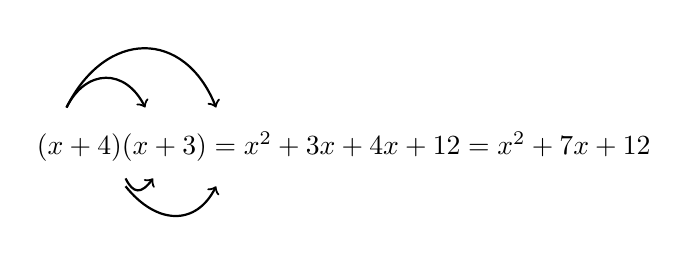
\begin{tikzpicture}
		\draw[black, thick, ->](0,0).. controls (0.25,0.5) and (0.75,0.5)..(1,0);
		\draw[black, thick, ->](0,0).. controls (0.5,1) and (1.5,1)..(1.9,0);
		\draw[black, thick, ->](0.75,-0.9).. controls (0.85,-1.1) and (0.95,-1.1)..(1.1,-0.9);
		\draw[black, thick, ->](0.75,-1).. controls (1.15,-1.5) and (1.65,-1.5)..(1.9,-1);
		\node at (-0.5,-0.5)[right]{ $(x+4)(x+3)=x^{2}+3x+4x+12=x^{2}+7x+12$};
	\end{tikzpicture}
\end{center}
\newpage
\question
Expand and simplify
\begin{multicols}{2}
	\begin{enumerate}[label=\normalsize \alph*)~~~]
		\item $(x + 3)(x - 1)$
		\item $(x + 7)(x - 4)$
		\item $(x - 4)(x + 2)$
		\item $(x - 3)(x - 6)$
			\end{enumerate}
	\end{multicols}
\questionend
\question
Expand and simplify
\begin{multicols}{2}
	\begin{enumerate}[label=\normalsize \alph*)~~~]
		\item $(x - 3)(5 - x)$
		\item $(2 - x)(4 + x)$
	\end{enumerate}
\end{multicols}
\questionend
\question
Expand and simplify
\begin{multicols}{2}
	\begin{enumerate}[label=\normalsize \alph*)~~~]
		\item $(2x + 3)(x - 1)$
		\item $(4x + 7)(2x + 3)$
		\item $(7x - 1)(2x - 1)$
		\item $(1 - 4x)(1 - 5x)$
	\end{enumerate}
\end{multicols}
\questionend
\question
Expand and simplify
\begin{multicols}{2}
	\begin{enumerate}[label=\normalsize \alph*)~~~]
		\item $(x+3)(x+3)$
		\item $(x +  5)^2$
		\item $(x - 1)^2$
		\item $(x-2)^2$
	\end{enumerate}
\end{multicols}
\questionend
\question
Expand and simplify
\begin{multicols}{2}
	\begin{enumerate}[label=\normalsize \alph*)~~~]
		\item $(x-1)(x+1)$
		\item $(x - 5)(x+ 5)$
		\item $(2x - 1)(2x+ 1)$
		\item $(3x +7)(3x -7)$
	\end{enumerate}
\end{multicols}
\questionend\vspace{-1cm}
\newpage
\question
Extension : Expand and simplify
\begin{multicols}{2}
	\begin{enumerate}[label=\normalsize \alph*)~~~]
		\item $(x-1)(x^2 + x + 1)$
		\item $(x + y - 5)(x + y+ 5)$
		\item $(x - y^3 + 1 )(x - y^3 - 1)$
		\item $(3x - 2y^5 - 7 )(3x - 2y^5 + 7)$
	\end{enumerate}
\end{multicols}
\questionend
		
\newpage
\section{Factorising to double brackets (quadratic factorising)}
To help us develop techniques to factorise quadratics, it is useful to do the number activity below.
\subsection{Sum Products }
The top box is the product of the two middle boxes and the bottom box is the sum.\\
Find the empty boxes.\\\\
% bottom , top , left , right
\sumproduct{}{$+54$}{}{$-6$}{1}
\sumproduct{}{ $-63$ }{$+7$}{}{2}
\sumproduct{$-22$}{}{$-16$}{}{3}\vspace{0cm}
The ones below can go either way round in the boxes\\
\sumproduct{$-1$}{$-12$}{}{}{4}
\sumproduct{$+5$}{$-6$}{}{}{5}
\sumproduct{$+1$}{$-6$}{}{}{6}\vspace{-0.5cm}\\
\sumproduct{$-10$}{$+21$}{}{}{7}
\sumproduct{$-8$}{$+16$}{}{}{8}
\sumproduct{$+13$}{$-30$}{}{}{9}\vspace{-0.5cm}\\
\sumproduct{$-5$}{$-150$}{}{}{10}
\sumproduct{$-2$}{$-3 \times 65$}{}{}{11}
\sumproduct{$+1$}{$-210$}{}{}{12}\vspace{-2cm}
\newpage
\subsection{Factorising}
So for an expression of the same structure, e.g $x^2+10x+21$\\
The $a$ and $b$ are two numbers that:
\begin{itemize}
	\item   \emph{Add to=10} 
	\item   \emph{Multiply to=21}
\end{itemize} 
Finding the factors of 21 , we get  3 and 7.
$$x^2+10x+21=(x+3)(x+7)$$
\question
Factorise the following:
\begin{multicols}{2}
	\begin{enumerate}[label=\normalsize \alph*)~~~]
\item $ x^2 + 7x + 6 $ 
\item $ x^2 + 12x + 32 $ 
\item $ x^2 - 5x + 6$ 
\item $ x^2 + 3x - 10 $ 
\item $ x^2 + 8x - 20 $ 
\item $ x^2 + 11x - 26$ 
\item $ x^2 - 10x +21 $ 
\item $ x^2 - 3x + 2 $ 
\item $ x^2 - 14x + 48$ 
\item $ x^2 - 5x - 84 $ 
\item $ x^2 - 6x - 16 $ 
\item $ x^2 - 4x - 32$ 
\item $ x^2 - 30 + x $ 
\item $ x^2 - 30 - x $ 
\item $ x^2 - 9x$ 
\item $ x^2 - 22x + 40 $ 
\item $ x^2 + 12x + 27 $ 
\item $ x^2 - 13x + 36$ 
\item $ x^2 - 18 - 3x $ 
\item $ 30x + x^2 + 225 $ 
\item $ 2x - 99 + x^2$ 
	\end{enumerate}
\end{multicols}
\questionend
\newpage
\section{Solving Quadratic Equations}
\subsection{Using factorised quadratics}
Consider the following equation: 
$$(x-6)(x+3)=0$$
To solve this equation, we do \underline{not} expand the brackets.\\
we can note that the equation is of the form:
\begin{align*}
	A \times B =0 ~~~~~~~~~~~~~~~ \text{where } A=(x-6) \text{ and } B=(x+3)
\end{align*}
And we can also note that if $A \times B = 0$, then either $A=0$ or $B=0$ \\\\
So $(x-6)(x+3)=0$ has \textbf{two} solutions.
\begin{align*}
	&(x-6)(x+3)=0\\
	x-6& = 0 \text{~~~~or~~~~} x+3=0\\
	\Rightarrow~~~~ x&=6  \text{~~~~or~~~~} x=-3
\end{align*}
\question
Solve the following:
\begin{multicols}{2}
	\begin{enumerate}[label=\normalsize \alph*)~~~]
		\item $(x-1)(x+7)=0$
		\item $(x - 5)(x+ 5)=0$
		\item $(x+11)(x+9)=0$
		\item $(x - 3)(x - 15)=0$
	\end{enumerate}
\end{multicols}
\question
Solve the following:
\begin{multicols}{2}
	\begin{enumerate}[label=\normalsize \alph*)~~~]
		\item $(3x-15)(2x+8)=0$
		\item $(2x - 8)(4x+ 1)=0$
		\item $(8x+10)(2x+9)=0$
		\item $(2x - 7)(2x - 15)=0$
	\end{enumerate}
\end{multicols}
\question
Solve the following:
\begin{multicols}{2}
	\begin{enumerate}[label=\normalsize \alph*)~~~]
		\item $3x(x+8)=0$
		\item $x(x+4)=0$
		\item $-3x(2x+9)=0$
		\item $x(2x - 15)=0$
	\end{enumerate}
\end{multicols}
\questionend
\newpage
\subsection{Using un-factorised quadratics}
To solve the equation:
$$x^2 + 3x -88 =0$$
\begin{align*}
	                          &&x^2 + 3x -88&=0&&\\
\textbf{factorise} &&(x-8)(x+11)&=0&&\\
                             &&x+8 = 0&\text{~~~~or~~~~} x+11=0&&\\
							&&x=-8  &\text{~~~~or~~~~} x=-11&&
\end{align*}

\question
\begin{multicols}{2}
	\begin{enumerate}[label=\normalsize \alph*)~~~]
\item $ x^2 + 7x + 6=0 $ 
\item $ x^2 + 12x + 32=0 $ 
\item $ x^2 - 5x + 6=0$ 
\item $ x^2 + 3x - 10=0 $ 
	\end{enumerate}
\end{multicols}
\question
\begin{multicols}{2}
	\begin{enumerate}[label=\normalsize \alph*)~~~]
	\item $ x^2 +6x =0$ 
	\item $ x^2 - 5x =0$ 
	\item $ x^2 - 18 - 3x =0$ 
	\item $ 2x - 99 + x^2=0$ 
	\end{enumerate}
\end{multicols}
\question
\begin{multicols}{2}
	\begin{enumerate}[label=\normalsize \alph*)~~~]
		\item $ x^2 + 0x -9 =0$ 
		\item $ x^2 - 0x -36 =0$ 
		\item $ x^2  - 25 =0$ 
		\item $ x^2 - 49=0$ 
	\end{enumerate}
\end{multicols}
\question
\begin{multicols}{2}
	\begin{enumerate}[label=\normalsize \alph*)~~~]
		\item $ x^2 - 6x + 9  =0$ 
		\item $ x^2 + 10x +25 =0$ 
		\item $ x^2  - 2x + 1 =0$ 
		\item $ x^2  + 2x + 1=0$ 
	\end{enumerate}
\end{multicols}
\questionend
\newpage
\subsection{Re-arranging into standard form}
If we get an equation with an $x^2$ as its highest power, we need to re-organise it into \textbf{standard form}
$$x^2 +bx +c =0$$
Once this is done, we can factorise and solve.\\\\
\textbf{(Example) Solve}: 
$$3=4x - x^2$$
\begin{align*}
\underline{\text{rearrange}} &&3=4x - x^2&&&\\
								&&3+x^2& =4x&&\\
                               &&3+x^2 -4x&=0&&\\
\underline{\text{standard form}}&&x^2 -4x+3&=0&&\\
\underline{\text{factorise}}&&(x-3)(x-1)&=0&&\\
							  &&x-3 = 0&\text{~~~~or~~~~} x-1=0&&\\
							  &&x=3  &\text{~~~~or~~~~} x=1&&
\end{align*}

\question
\begin{multicols}{2}
	\begin{enumerate}[label=\normalsize \alph*)~~~]
		\item $ -26  = 11x -x^2$ 
		\item $ 18x + x^2 = -45$ 
		\item $  42=x^2 - 11x$ 
		\item $ x^2 + 225=30x$ 
	\end{enumerate}
\end{multicols}
\question
\begin{multicols}{2}
	\begin{enumerate}[label=\normalsize \alph*)~~~]
			\item $ x(x-2)=15$ 
			\item $ (x-3)^2= 25$ 
			\item $  (x-4)(x-6)=8$ 
			\item $ (x-3)(x+2)=4x$ 
			\item $  (x+2)(x+7)=(x+5)(x+7)$ 
			\item $ \displaystyle x+3 = \frac{12}{x+4}$ 
	\end{enumerate}
\end{multicols}
\questionend
\newpage
\subsection{Word questions}
\question
	\begin{enumerate}[label=\normalsize \alph*)~~~]
		\item When a number is squared, and then 1 is subtracted, the result is 8.
		\begin{enumerate}[label=\normalsize \roman*)]
			\item Write this information down as a quadratic equation.
			\item Solve the equation to work out the two possible numbers.
		\end{enumerate}
	\item A number is squared, and then added to the original number. The result is 20.
	\begin{enumerate}[label=\normalsize \roman*)]
	\item Write this information down as a quadratic equation.
	\item Solve the equation to work out the two possible numbers.
		\end{enumerate}
	\item When a number $x$, is multiplied by a number 4 less than $x$, the result is 12.\\
	What two numbers have this property?
	\item Squaring a number gives the same result as multiplying the number by 8, and then subtracting 12.
	\begin{enumerate}[label=\normalsize \roman*)]
		\item Write this information down as a quadratic equation.
		\item Solve the equation to work out the two possible numbers.
	\end{enumerate}
	\item When the result of adding 2 to a number is multiplied by the result of subtracting  2 
	from the same number, the answer is 21. \\
	What two numbers have this property?
	\end{enumerate}
\questionend
\newpage
\section{Revision}
\begin{enumerate}
	\item Simplify
\begin{multicols}{2}
	\begin{enumerate}[label=\normalsize \alph*)~~~]
			\item $ 4x +x$ 
			\item $10x + y -4 -5x$ 
			\item $4x^2 +x -2x^2 + 3x$ 
			\item $ 2abc + 4a - 5b + c +abc - 2a + 3b$ 
			\item $ \displaystyle \frac{32x^6}{24x^2}$ 
			\item $ \displaystyle \frac{4x^2y^3}{2xy^4}$ 
			\item $ \left( 2x^2 \right)^3$ 
			\item $ \left( 4x^2y^3 \right)^2$ 
	\end{enumerate}
\end{multicols}
\item Expand
\begin{multicols}{3}
	\begin{enumerate}[label=\normalsize \alph*)~~~]
			\item $ 3x(x+2)$ 
			\item $5(2p-q)$ 
			\item $x(x-3) + 8(x-1)$ 
			\item $ x(2x-3) - 2(x+2)$ 
			\item $ (8x-3)(x+1)$ 
			\item $ (2x + 3)(5-3x)$ 
			\item $ (2x-1)(2x+1)$ 
	\end{enumerate}
\end{multicols}
\item Factorise (one bracket)
\begin{multicols}{2}
	\begin{enumerate}[label=\normalsize \alph*)~~~]
		\item $ 4a + 4b$ 
		\item $5x + 20y$ 
		\item $7x - 3x^2$ 
		\item $ 24xy^2z - 18x^3yz$ 
	\end{enumerate}
\end{multicols}
\item Factorise (two brackets)
\begin{multicols}{2}
	\begin{enumerate}[label=\normalsize \alph*)~~~]
		\item $ x^2 + 8x + 15$ 
		\item $x^2 - 2x -15$ 
		\item $x^2 - 15x +56$ 
		\item $ x^2 + 5x -36$ 
	\end{enumerate}
\end{multicols}
\item Factorise (two brackets)
\begin{multicols}{3}
	\begin{enumerate}[label=\normalsize \alph*)~~~]
		\item $ x^2 -16$ 
		\item $x^2 - 121$ 
		\item $x^2 - 1$ 
	\end{enumerate}
\end{multicols}
\item Solve (Linear equations)
\begin{multicols}{2}
	\begin{enumerate}[label=\normalsize \alph*)~~~]
		\item $ x+3 =14$ 
		\item $\displaystyle \frac{x}{5} = -2$ 
		\item $\displaystyle \frac{x-4}{6} = -3$ 
		\item $12 - 3x=36 + 5x$ 
	\end{enumerate}
\end{multicols}
\item Solve (Quadratic equations)
\begin{multicols}{2}
	\begin{enumerate}[label=\normalsize \alph*)~~~]
		\item $ (x-6)(x-3) = 0$ 
		\item $3x(x+2) = 0$ 
		\item $x^2 +8x - 5 = 4$ 
		\item $2x(4-x)=6$ 
			\item $(x-3)(x+2)=4x$ 
	\end{enumerate}
\end{multicols}
\end{enumerate}
\newpage
\section{Practice Test}
\begin{enumerate}
	\item  Simplify
\begin{multicols}{2}
	\begin{enumerate}[label=\normalsize \alph*)~~~, itemsep=0.4cm]
		\item $ 2x^5 + 3x - 6x + 5x^5 + 2$ 
		\item $3pq + 5qp + 7pr - 2qr$ 
		\item $8x^2 \times 4x^4$ 
		\item $2abc \times 3a^2b \times 5a^2c^6$ 
		\item $ \left( 6t^4 \right)^3$ 
		\item $\displaystyle \frac{ 125 d^{10} e^4}{ 25 d^5 e^6}$
		\item $\displaystyle \frac{ 32 j^{11} k^8}{ 24 j^{14} k^{10} l}$
	\end{enumerate}
\end{multicols}
\item Expand and simplify if possible
\begin{multicols}{2}
	\begin{enumerate}[label=\normalsize \alph*)~~~,  itemsep=0.4cm]
		\item $3(2x +9)$ 
		\item $4x(8y-3) - 2(4x+7)$ 
		\item $(x+5)(x-3)$ 
		\item $(x-8)^2$ 
	\end{enumerate}
\end{multicols}
\item Factorise
\begin{multicols}{2}
	\begin{enumerate}[label=\normalsize \alph*)~~~,  itemsep=0.4cm]
		\item $14c + 21d$ 
		\item $36ab^2c^5 - 18b^4c^3$ 
		\item $x^2 + 10x +21$ 
		\item $x^2 - 5x -14$ 
		\item $x^2 - 4x-165$ 
		\item $3x^2 - 75$ 
	\end{enumerate}
\end{multicols}
\item Solve
\begin{multicols}{2}
	\begin{enumerate}[label=\normalsize \alph*)~~~, itemsep=0.4cm]
		\item $4x - 7 =21$ 
		\item $\displaystyle \frac{25x-5}{8} = 15$ 
		\item $5(x-11) =35$ 
		\item $2x+3 = 6x -33$ 
		\item $(x-3)(x+5)= 0$ 
		\item $x^2 + 8x -33=0$ 
		\item $x^2  - 23x +102=0$ 
	\end{enumerate}
\end{multicols}
\item The sum of two consecutive odd numbers is 88. Form an equation and use it to find the numbers. 
\item A piece of land is a rectangle and the length is eight metres longer than twice its width.
\begin{enumerate}
	\item Draw a diagram
	\item Find expressions for the area and the perimeter.
	\item The area of the land is 640$m^2$, find the length and width of the land.
	\item Find the perimeter of the land.
\end{enumerate}
\end{enumerate}






\end{document}

